%% March 2018
%%%%%%%%%%%%%%%%%%%%%%%%%%%%%%%%%%%%%%%%%%%%%%%%%%%%%%%%%%%%%%%%%%%%%%%%%%%%
% AGUJournalTemplate.tex: this template file is for articles formatted with LaTeX
%
% This file includes commands and instructions
% given in the order necessary to produce a final output that will
% satisfy AGU requirements, including customized APA reference formatting.
%
% You may copy this file and give it your
% article name, and enter your text.
%
%%%%%%%%%%%%%%%%%%%%%%%%%%%%%%%%%%%%%%%%%%%%%%%%%%%%%%%%%%%%%%%%%%%%%%%%%%%%
% PLEASE DO NOT USE YOUR OWN MACROS
% DO NOT USE \newcommand, \renewcommand, or \def, etc.
%
% FOR FIGURES, DO NOT USE \psfrag or \subfigure.
% DO NOT USE \psfrag or \subfigure commands.
%%%%%%%%%%%%%%%%%%%%%%%%%%%%%%%%%%%%%%%%%%%%%%%%%%%%%%%%%%%%%%%%%%%%%%%%%%%%
%
% Step 1: Set the \documentclass
%
% There are two options for article format:
%
% PLEASE USE THE DRAFT OPTION TO SUBMIT YOUR PAPERS.
% The draft option produces double spaced output.
%

%% To submit your paper:
\documentclass[draft,linenumbers]{agujournal2018}
\usepackage{apacite}
\usepackage{natbib}
\usepackage{amsmath}
\usepackage{multirow}
\usepackage{threeparttable}
\usepackage{url} %this package should fix any errors with URLs in refs.

\linespread{1.5}

%%%%%%%
\usepackage[inline]{trackchanges}
\addeditor{AS}
\addeditor{EC}
% uncomment the line above to use the TrackChanges package to mark revisions if needed.
% The trackchanges package adds five new LaTeX commands:
%
%  \note[editor]{The note}
%  \annote[editor]{Text to annotate}{The note}
%  \add[editor]{Text to add}
%  \remove[editor]{Text to remove}
%  \change[editor]{Text to remove}{Text to add}
%
% complete documentation is here: http://trackchanges.sourceforge.net/
%%%%%%%

\draftfalse

% Now, type in the journal name: \journalname{<Journal Name>}

% ie, \journalname{Journal of Geophysical Research}
%% Choose from this list of Journals:
%
% JGR-Atmospheres
% JGR-Biogeosciences
% JGR-Earth Surface
% JGR-Oceans
% JGR-Planets
% JGR-Solid Earth
% JGR-Space Physics
% Global Biochemical Cycles
% Geophysical Research Letters
% Paleoceanography
% Radio Science
% Reviews of Geophysics
% Tectonics
% Space Weather
% Water Resource Research
% Geochemistry, Geophysics, Geosystems
% Journal of Advances in Modeling Earth Systems (JAMES)
% Earth's Future
% Earth and Space Science
% Geohealth
%

\journalname{<enter journal name here>}


\begin{document}

%% ------------------------------------------------------------------------ %%
%  Title
%
% (A title should be specific, informative, and brief. Use
% abbreviations only if they are defined in the abstract. Titles that
% start with general keywords then specific terms are optimized in
% searches)
%
%% ------------------------------------------------------------------------ %%

% Example: \title{This is a test title}

\title{Stress concentration due to upper mantle heterogeneity in the Central and Southeastern US seismic zones} 
%% ------------------------------------------------------------------------ %%
%
%  AUTHORS AND AFFILIATIONS
%
%% ------------------------------------------------------------------------ %%

% Authors are individuals who have significantly contributed to the
% research and preparation of the article. Group authors are allowed, if
% each author in the group is separately identified in an appendix.)

% List authors by first name or initial followed by last name and
% separated by commas. Use \affil{} to number affiliations, and
% \thanks{} for author notes.
% Additional author notes should be indicated with \thanks{} (for
% example, for current addresses).

% Example: \authors{A. B. Author\affil{1}\thanks{Current address, Antartica}, B. C. Author\affil{2,3}, and D. E.
% Author\affil{3,4}\thanks{Also funded by Monsanto.}}

\authors{Arushi Saxena, Eunseo Choi, Christine A. Powell and Khurram S. Aslam}


% \affiliation{1}{First Affiliation}
% \affiliation{2}{Second Affiliation}
% \affiliation{3}{Third Affiliation}
% \affiliation{4}{Fourth Affiliation}

\affiliation{}{Center for Earthquake Research and Information, University of Memphis}
%(repeat as many times as is necessary)

%% Corresponding Author:
% Corresponding author mailing address and e-mail address:

% (include name and email addresses of the corresponding author.  More
% than one corresponding author is allowed in this LaTeX file and for
% publication; but only one corresponding author is allowed in our
% editorial system.)

% Example: \correspondingauthor{First and Last Name}{email@address.edu}

\correspondingauthor{Arushi Saxena}{asaxena@memphis.edu}

%% Keypoints, final entry on title page.

% Example:
% \begin{keypoints}
% \item	List up to three key points (at least one is required)
% \item	Key Points summarize the main points and conclusions of the article
% \item	Each must be 100 characters or less with no special characters or punctuation
% \end{keypoints}

%  List up to three key points (at least one is required)
%  Key Points summarize the main points and conclusions of the article
%  Each must be 100 characters or less with no special characters or punctuation

\begin{keypoints}
\item Numerical models based on a recent tomography reveals stress concentration from the upper mantle heterogeneity at the seismic zones in Central and Eastern US
\item Coulomb stress increases at the Eastern Tennessee and New Madrid seismic zones due to sinking lithospheric root
\item Favorable preexisting faults along with deep upper mantle  heterogeneity could lead to earthquake generation in Central and Eastern US
\end{keypoints}

%% ------------------------------------------------------------------------ %%
%
%  ABSTRACT
%
% A good abstract will begin with a short description of the problem
% being addressed, briefly describe the new data or analyses, then
% briefly states the main conclusion(s) and how they are supported and
% uncertainties.
%% ------------------------------------------------------------------------ %%

%% \begin{abstract} starts the second page

\begin{abstract}
Sources of stresses responsible for earthquakes occurring in the Central and Eastern US (CEUS) must include not only far-field plate boundary forces but also various local contributions. In this study, we model stress distributions due to heterogeneities in the upper mantle beneath CEUS including a high-velocity feature identified as a lithospheric root in a recent regional P wave tomography. A temperature field is converted from the tomography and the corresponding viscosity field is acquired using temperature-dependent dislocation and diffusion creep rheology. We retrieve velocity and stress fields from instantaneous 3D numerical models that take the converted temperature and viscosity fields as inputs. We isolate all the heterogeneity deeper than 200 km in one model setup and additionally, a high density feature interpreted as lithospheric root in another. Model results attributed to all the upper mantle heterogeneity show high differential stress and Coulomb stress at the optimal fault orientations of the seismic zones. However, the sole effect of root show stress concentration only at the seismic zones in the vicinity of the root: Eastern Tennessee Seismic Zone and the northeast arm of the New Madrid Seismic Zone. We also calculate the Coulomb stress from our models at a range of theoretical fault orientations and dips. Our findings suggest that the upper mantle structure below the CEUS contributes in increasing the stress field, promoting earthquake generation at preexisting faults in the region's seismic zones. %Moreover, these heterogeneities increase the Coulomb stress at preexisting faults in the seismic zones, generating earthquakes.

\end{abstract}


%% ------------------------------------------------------------------------ %%
%
%  TEXT
%
%% ------------------------------------------------------------------------ %%


\section{Introduction}
    The Central and Eastern US (CEUS) is characterized by a number of intraplate seismic zones including the New Madrid Seismic Zone (NMSZ), the Eastern Tennessee Seismic Zone (ETSZ), the South Carolina Seismic Zone (SCSZ), the Giles County Seismic Zone (GCSZ) and the Central Virginia Seismic Zone (CVSZ) (Fig.~\ref{figone}). 
    
    Tectonic setting of the CEUS includes complex fault systems formed by two continent-scale episodes of rifting and collision~\citep[e.g.,][]{keller1983role, hoffman1989precambrian, thomas2006tectonic}. Within these systems, optimally oriented faults with respect to the present-day regional or local stresses can get reactivated, generating earthquakes~\citep[e.g.,][]{zoback1992stress, hurd2012intraplate}. Far from the tectonic plate boundaries with low geodetically detectable strain rates~\citep{Boyd_2015}, local stress contributions can play an important role in the eathquake generation at the CEUS. 
    
    Many studies have proposed mechanisms in the CEUS for stress concentration due to the local effects but the origin of these pertubations considered by them is diverse involving both crustal and upper mantle heterogeneity. \citet{Kenner_2000a} proposed the presence of a weaker lower crustal zone within an elastic lithosphere that acts as a local source of stress concentration. \citet{Pollitz_2001} suggested a geodynamic model for NMSZ consisting of a sinking mafic body in the weakened lower crust that can transfer stress into the overlying elastic crust. \citet{levandowski2016dense} showed that a high density lower crust below the NMSZ interferes constructively with the far-field tectonic stress causing optimal stress orientations for earthquake generation.  Although the seismogenic depths in the CEUS is located in the upper to middle crust (5 to 30 km) \citep{vlahovic1998et1d, johnston1996seismic, mazzotti2010state}, deeper mantle structures can also make a significant contribution to the generation of  earthquakes~\citep[e.g.,][]{forte2007descent, li2007stress, chen2014crust, nyamwandha2016joint, zhan2016stress}. \citet{forte2007descent} showed that stress concentration below the NMSZ can be produced by the descent of the Farallon slab using a global geodynamic and seismic tomography based numerical model. \citet{li2007stress} showed that lateral heterogeneity in the lithosphere below the CEUS can concentrate stress. \citet{chen2014crust} and \citet{nyamwandha2016joint} independently observed low P velocity zone at 50-200 km depths below the NMSZ interpreted as a weak zone which acts as conduit for stress transfer into the crust. \citet{zhan2016stress} determined that higher upper mantle temperatures, based on a regional tomography \citep{pollitz2014seismic}model, will focus stress in the crust of the NMSZ.
    
    % , with special attention given to the heterogeneities beneath the NMSZ.

    %
\begin{figure}[ht]
    \centering
    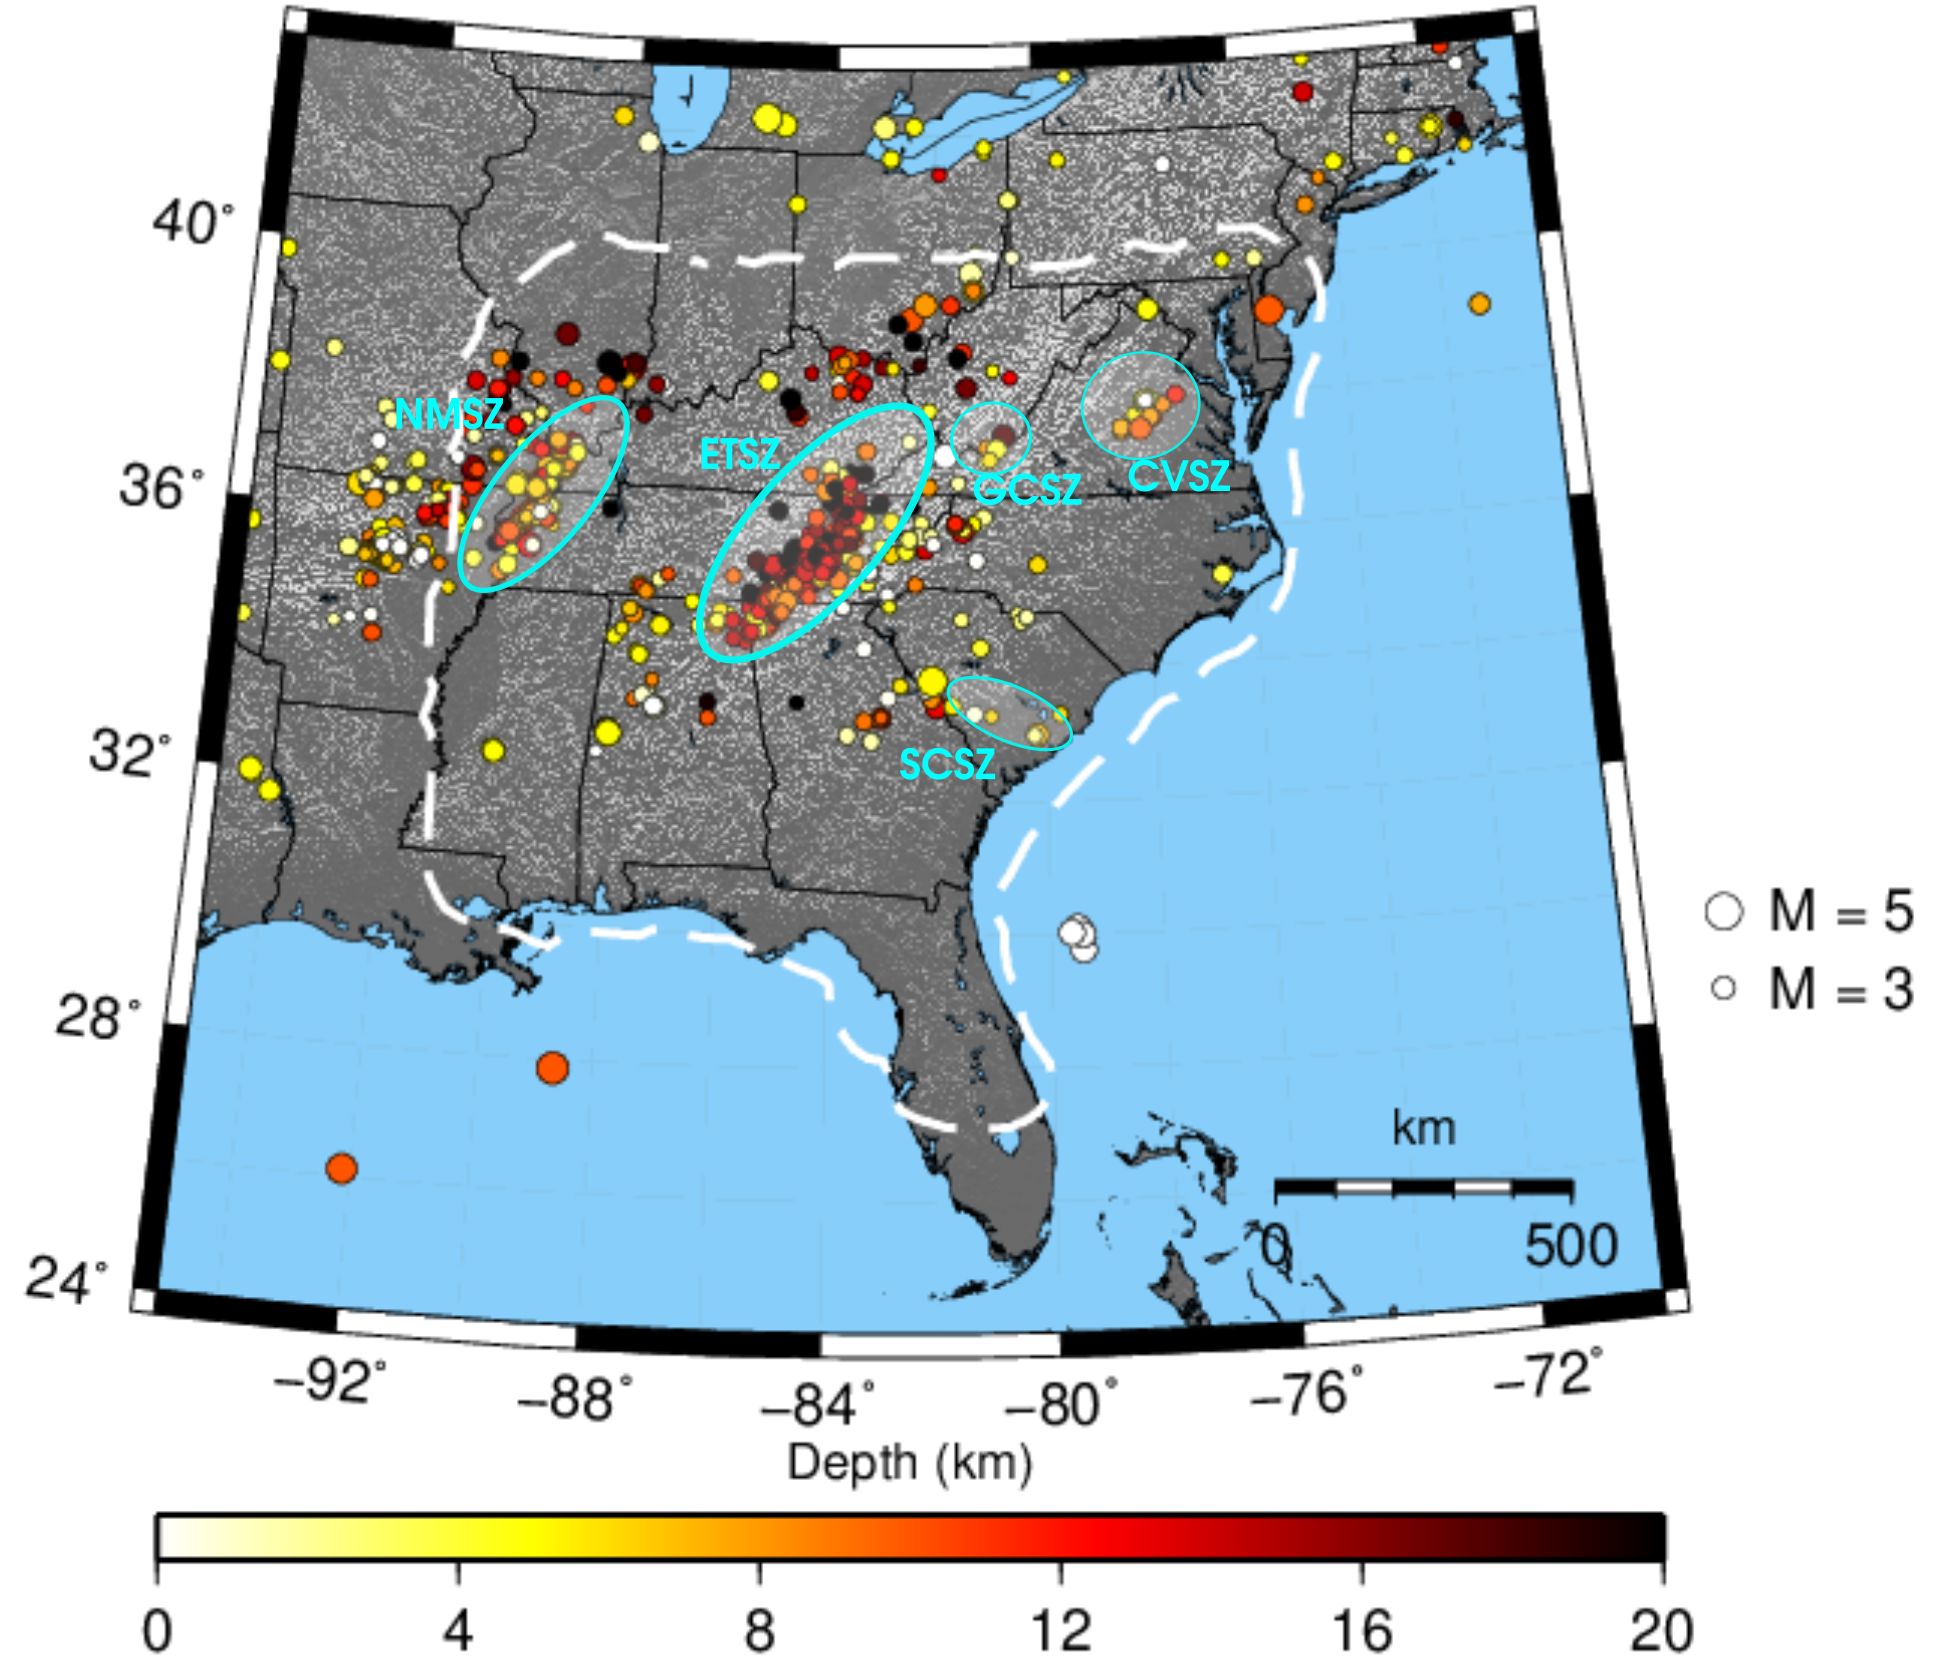
\includegraphics[width=20pc]{figures/seismicity_new.png}
    \caption{ A shaded relief map of the study area including the central and southeastern US seismic zones: New Madrid Seismic Zone (NMSZ), Eastern Tennessse Seismic Zone (ETSZ) South Carolina Seismic Zone (SCSZ), Giles County Seismic Zone (GCSZ) and Central Virginia Seismic Zone (CVSZ). White dashed line represents the well sampled region in the tomography results by~\citet{Biryol_2016} at depth 130 km. The earthquakes that occurred over the period December 2011 - December 2018 and had $M_{w} > 2.5$ are plotted as colored circles. The size and color of a circle represent the event's magnitude and depth. The earthquake catalogue is obtained from the United States Geological Survey at \url{https://earthquake.usgs.gov/earthquakes/search/}.}
    \label{figone}
 \end{figure}
 %
   
%Several past studies focusing on the NMSZ have suggested that the crustal structure of this seismic zone causes stress concentration~\citep{Kenner_2000a, Pollitz_2001, levandowski2016dense}. \citet{Kenner_2000a} proposed the presence of a weaker lower crustal zone within an elastic lithosphere that acts as a local source of stress concentration. \citet{Pollitz_2001} suggested a geodynamic model for NMSZ consisting of a sinking mafic body in the weakened lower crust that can transfer stress into the overlying elastic crust. \citet{levandowski2016dense} showed that a high density lower crust below the NMSZ interferes constructively with the far-field tectonic stress causing optimal stress orientations for earthquake generation.
    
     Similar considerations of crustal and mantle stress sources are yet to be made for other CEUS seismic zones such as the ETSZ, SCSZ, GCSZ and CVSZ. In a recent high-resolution P wave tomography study, \citet{Biryol_2016} found positive velocity anomalies in the upper mantle beneath the area in between the ETSZ and the NMSZ at depths 200 to 660 km, and interpreted them as foundering lithosphere. They further speculated that, since the seismic zones like the NMSZ and ETSZ coincide with the boundary of lithosphere thinned by the delamination, they are weakened by the underlying hot asthenosphere and thus prone to seismicity. 
    
    In this study, we investigate the effects of the upper mantle heterogeneities found in~\citet{Biryol_2016}'s tomography on the seismicity in the CEUS. We compute stress fields arising from density and strength variations converted from the tomography using instantaneous three-dimensional (3D) mantle flow models. %explaining the location of seismic zones and assessing the sources of their initiation \citep{zoback1992stress, king1994static, stein1999role, bowman2001accelerating}. 
Previous studies have utilized changes in differential stress~\citep[e.g.,][]{baird2010relationship, zhan2016stress}) and deviatoric stress ~\citep[e.g.,][]{levandowski2016dense}) to correlate the highs with the observed intraplate seismicity. These stress indicators are useful for  observing the stress distribution within the brittle crust. Under the stress field, the tendency of a fault to slip is determined by the Coulomb failure criterion which accounts for the fault strength and the stresses on that fault geometry~\citep{king1994static, freed2005earthquake, li2007stress}. 

\section{Seismic tomography}
We briefly summarize the seismic tomography results by \citet{Biryol_2016} with the resolution and the uncertainties associated with it before explaining our numerical models and results.

    The tomography study by \citet{Biryol_2016} is based on direct P and PKPdf residual travel times with respect to the IASP91 earth model \citep{kennett1991traveltimes}. The data is collected from 514 stations in the study region (Fig. \ref{figone}) for 753 teleseismic earthquakes occurring between 2011 to 2015 with moment magnitude, $Mw > 5.5$. The discretized model has a lateral extent of 30 km in the center and 45 km along the boundary of the domain. The depth extent of the grid is from 36 km to 915 km and consists of 21 layers, but we are only interested in the features extending down to 660 km for this study. They use the tomographic inversion algorithm by \citet{schmandt2010seismic} along with optimal smoothing and damping constraints to minimize their model norm and data misfit (described in detail in the supplementary information by \citet{Biryol_2016}). Only model nodes with high quality (hit points) are used and therefore model results at 36 km depth are not interpreted due to lower quality.
    
    \citet{Biryol_2016} verify their inversion results after robust resolution tests. The checkerboard and feature recovery tests indicate vertical smearing at shallow depths due to near vertical incidence of the teleseismic raypaths and amplitude loss by about 40 \% in the center of the model. Their calculated lateral resolution in the center is about 40 km going to 60 km towards the bottom of the domain while the vertical resolution  is around 50 km at the top and extends to 65 km at the bottom. They observe some artifacts due to smearing but have overall confidence on the large magnitude ($> 1\%$) and dimensional features. The locations of the smaller dimensional features ($\sim$ 100 km) are recovered in the synthetic resolution tests but their outline is smeared laterally and vertically. The well sampled region  in the tomographic inversion a after synthetic tests along with the high velocity anomaly (mean amplitude of 1.9\%) is shown in Fig. \ref{fig_tomo}. It is noted that this feature starts at an approximate depth $\sim$ 200 km with lateral dimensions of $1^\circ$ and extends to 660 km where it widens to about $3^\circ$. Because of its large amplitude and dimensions, the foundering lithospheric root is well resolved in their feature tests and therefore, reliable for our numerical model inputs. 

\begin{figure}[ht]
    \centering
    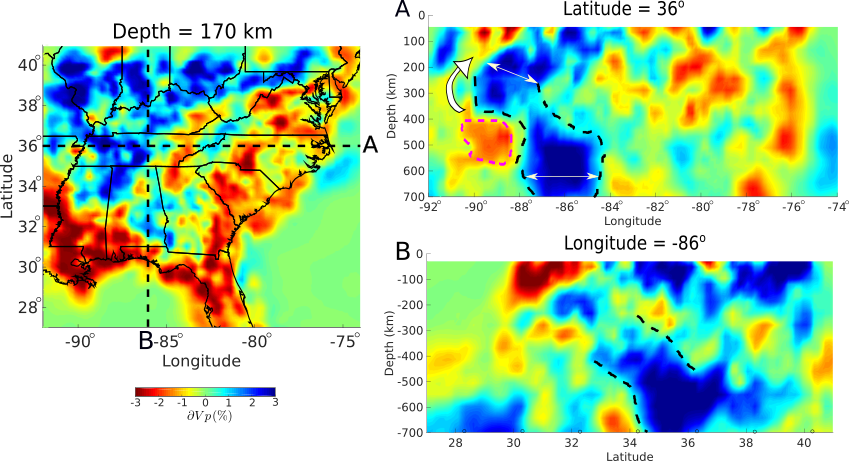
\includegraphics[width=\linewidth]{figures/figure_tomography.png}
    \caption{P wave tomography results from \citep{Biryol_2016} at depth layer 170 km along with latitude and longitude profiles A and B. Dashed line in the profiles marks the approximate dimensions of the high density anomaly interpreted as lithospheric foundering. }
    \label{fig_tomo}
 \end{figure}

\section{Methodology}
    Inputs for a mantle flow model include temperature and density fields, and the velocity anomalies are converted to them with the effects of anelasticity, compositional variations and phase changes taken into account. The effective rheology is assumed to be a combination of diffusion and dislocation creep. To make a meaningful interpretation of the presence of deeper heterogeneity, we use a reference model with laterally homogeneous temperatures at depths $>$ 200 km, with respect to which we calculate differential stress and Coulomb stress changes for different fault geometries. Since we are interested in the effects of the high-velocity anomalies interpreted as foundering (\citep{Biryol_2016}), we also examine dynamic topography, caused by the mantle flow induced by the sinking denser material. 
    
\subsection{Temperature Calculations} \label{temp_var}
    Converting seismic tomography for the mantle to a temperature field is commonly regarded as a non-linear problem due to the shear anelasticity of seismic waves \citep{minster1981model, karato1993importance, sobolev1996upper, Goes_2000, artemieva2004shear} and non-linear sensitivity of elastic moduli and their pressure derivatives to temperature \citep{duffy1989seismic, anderson1992high, Cammarano2003, stixrude2005thermodynamics}. The presence of melt or water may also introduce non-linearity in temperature effects on seismic velocities~\citep{Karato_1998} but these effects are not considered in this study for simplicity and lack of high heat flow and other substantial evidence for melting in this region of the  mantle~\citep{blackwell2006assessment}. We follow the approach given by \citet{Cammarano2003} to calculate temperature given the velocity anomalies, while incorporating the effects of anharmonicity (composition) (\ref{anh}) , anelasticity (\ref{anel}) and the phase transition at the 410 km boundary. The calculated temperatures and the corresponding velocity anomalies at depths of 200 km and 605 km are shown in Fig. \ref{fig_temp}. We describe our calculations in detail in Appendix A. 
%
\begin{figure}[ht]
    \centering
    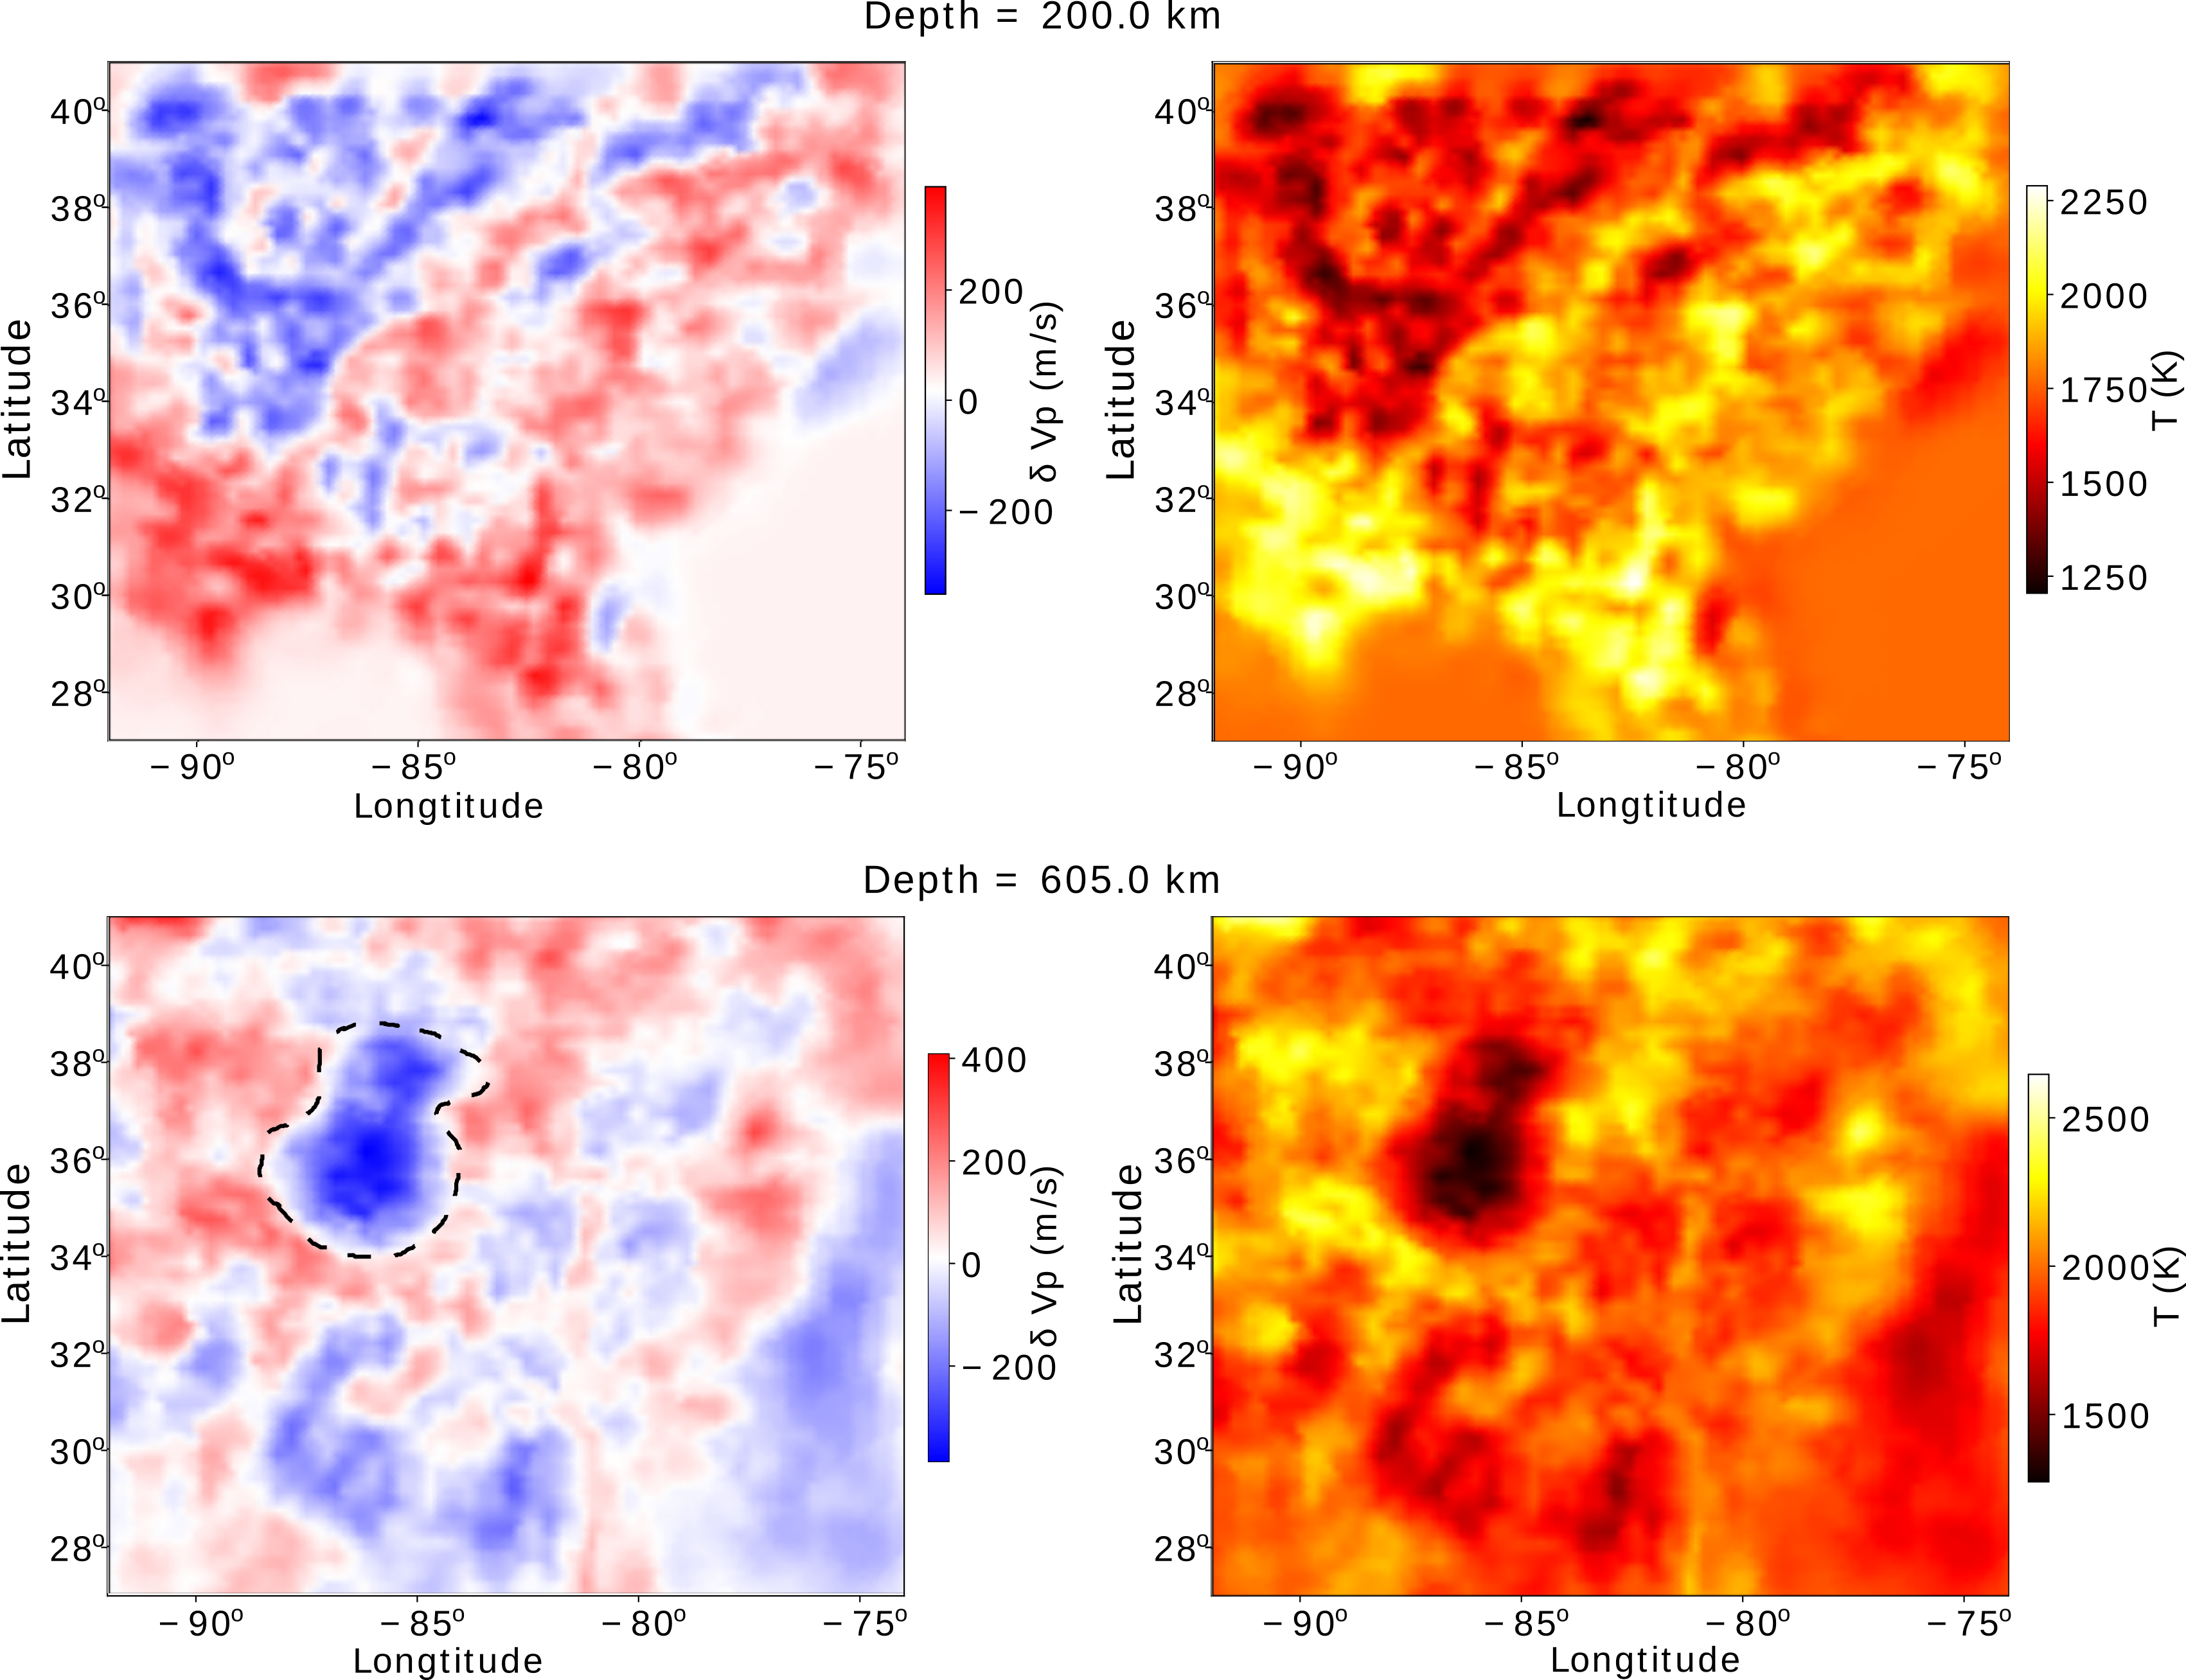
\includegraphics[width=0.75\linewidth]{figures/figure_temp.png}
    \caption{Temperatures (right) at depths of 200 and 605 km calculated from P wave anomalies (left) accounting for compositional variations, attenuation and the phase transformation at 410 km. Black dotted line marks the probable boundary of the high velocity structure interpreted as a foundering root by \citet{Biryol_2016}, see Fig. \ref{fig_model} for detailed structure outline.}
    \label{fig_temp}
 \end{figure}

Our approach has some differences from that of~\citet{Cammarano2003}. We invert velocity anomalies, not absolute velocities, for temperatures assuming a reference geotherm $T_o$. Our results involve errors due to uncertainties in the reference geotherm but it is sufficient to evaluate the heterogeneity in the temperature since same error propagated laterally. Another difference is that we use the Voigt (constant strain) averaging scheme to calculate elastic moduli and density of the composite mineral, which overestimates the converted values \citep{watt_1976}, instead of Hashin Shtrikman scheme.Seismic velocities calculated using the reference elastic moduli and composition using Voigt (upper bound) and Reuss (lower bound) averaging and find less than 0.2 \% difference in the values. Since this error is within the range of the tomography error \citep{Biryol_2016}, we use the Voigt scheme for simplicity. Finally, elastic moduli at high pressures are extrapolated using second-order accuracy instead of third-order, for simplicity in implementation of inversion.  

To calculate anharmonic effects on seismic velocity (\ref{anh}), we use the data on bulk modulus (K), shear modulus (G) and density ($\rho$) at reference mineral composition from \citet{Cammarano2003}, the geotherm ($T_o$) compiled from \citet{Goes_2002} for lithospheric (i.e., $<$ 200 km) depths and for greater depths from \citet{turcotte2014geodynamics}, and thermal expansivity ($\alpha$) from \citet{saxena_data} (see Table \ref{table1}). We assume a reference composition of harzburgite for the craton, i.e. 83 \% olivine (ol), 15 \% orthopyroxene (opx), 2 \% garnet (gt) \citep{mcdonough1998mineralogy} for depths 40 km to 410 km or pressure (P) $<$ 12.5 GPa. While at depths 410 km to 660 km, we use reference composition as 60 \% Mg-wadsleyite and 40 \% Majorite  \citep{haggerty1995upper}. We use Burnman \citep{cottaar2014burnman} to calculate the mantle adiabat with potential temperature $1300^o$ C for P $<$ 12.5 GPa, which is appropriate for continental lithosphere \citep{rudnick1998thermal} and $1600^o$ for P $>$ 12.5 GPa \citep{katsura2010adiabatic}. 

Anelasticity is implemented using the values given by \citet{sobolev1996upper} for their model 2 (pressure dependence on activation enthalpy in calculating attenuation, see \ref{anel}). We use the frequency for teleseismic tomography as 1 Hz in attenuation. We do not include the effects of melting in attenuation for the reasons discussed earlier.

Both anharmonic and anelastic effects on seismic velocity, discontinuous at the 410 km phase transition, are added to invert seismic anomalies for temperature. We start with an initial guess for temperature and iterate the value until we minimize the difference with the observed seismic anomalies following the newton-raphson approach for all the observational points. We also calculate temperatures accounting for uncertainties in the elastic moduli and its temperature derivatives (given in \citet{Cammarano2003}) and compare it with the results obtained here using their mean values given in Table \ref{table1}. Taking the maximum values of the elastic parameters reduces the temperature sensitivity such that the negative (positive) velocity anomaly decreases (increases) temperature by smaller ($\pm$ 90 K) magnitude. On the other hand, minimum parameter values increase the temperature sensitivity, and therefore the range of temperatures obtained, by $\sim$ 180 K. 

\subsection{Model Setup}
    We calculate the stress field associated with an instantaneous viscous mantle flow, which in turn is driven by thermal buoyancy arising from the heterogeneous temperature distribution converted from the P wave tomography by \citet{Biryol_2016} as described above. Model inputs, density and viscosity distributions, are computed based on the converted temperatures. 
    
    We use ASPECT version 2.0.0 for the mantle flow and stress calculations~\citep{heister_aspect_methods2,KHB12,aspect-doi-v2.0.0}, which solves the conservation of mass, momentum and energy equations using the finite element method. Fig \ref{fig_model} shows the model domain and the viscosity computed based on the temperature distribution. The domain is bounded laterally by longitudes 71$^\circ$W to 95.5$^\circ$W and latitudes 23$^\circ$N to 43$^\circ$N. The depth range of the model is from 0 to 660 km. Since the tomography model considers only the mantle starting from a depth of 40 km, we assume homogeneous material properties in the top 40 km-thick crust layer (i.e. temperature, density and viscosity are 500 $^{\circ}$C, 2900 kg/m$^{3}$ and  5x10$^{24}$Pa$\cdot$s). Our interest only in mantle stress sources justifies this assumption of a homogeneous crust. The domain is discretized into 512000 hexahedral elements such that the resolution is comparable with the tomography resolution: $0.15^\circ$ in longitude, $0.125^\circ$ in latitude and 35 km in depth. Although, the mantle structures seen in the tomography model are well resolved in our geodynamic model with this resolution, we also ran simulations with a finer grid (2048000 elements). Because differences in the results were small (relative error of 2\%), we consistently used the coarser mesh in this study for computational efficiency.
%
\begin{figure}[ht]
    \centering
    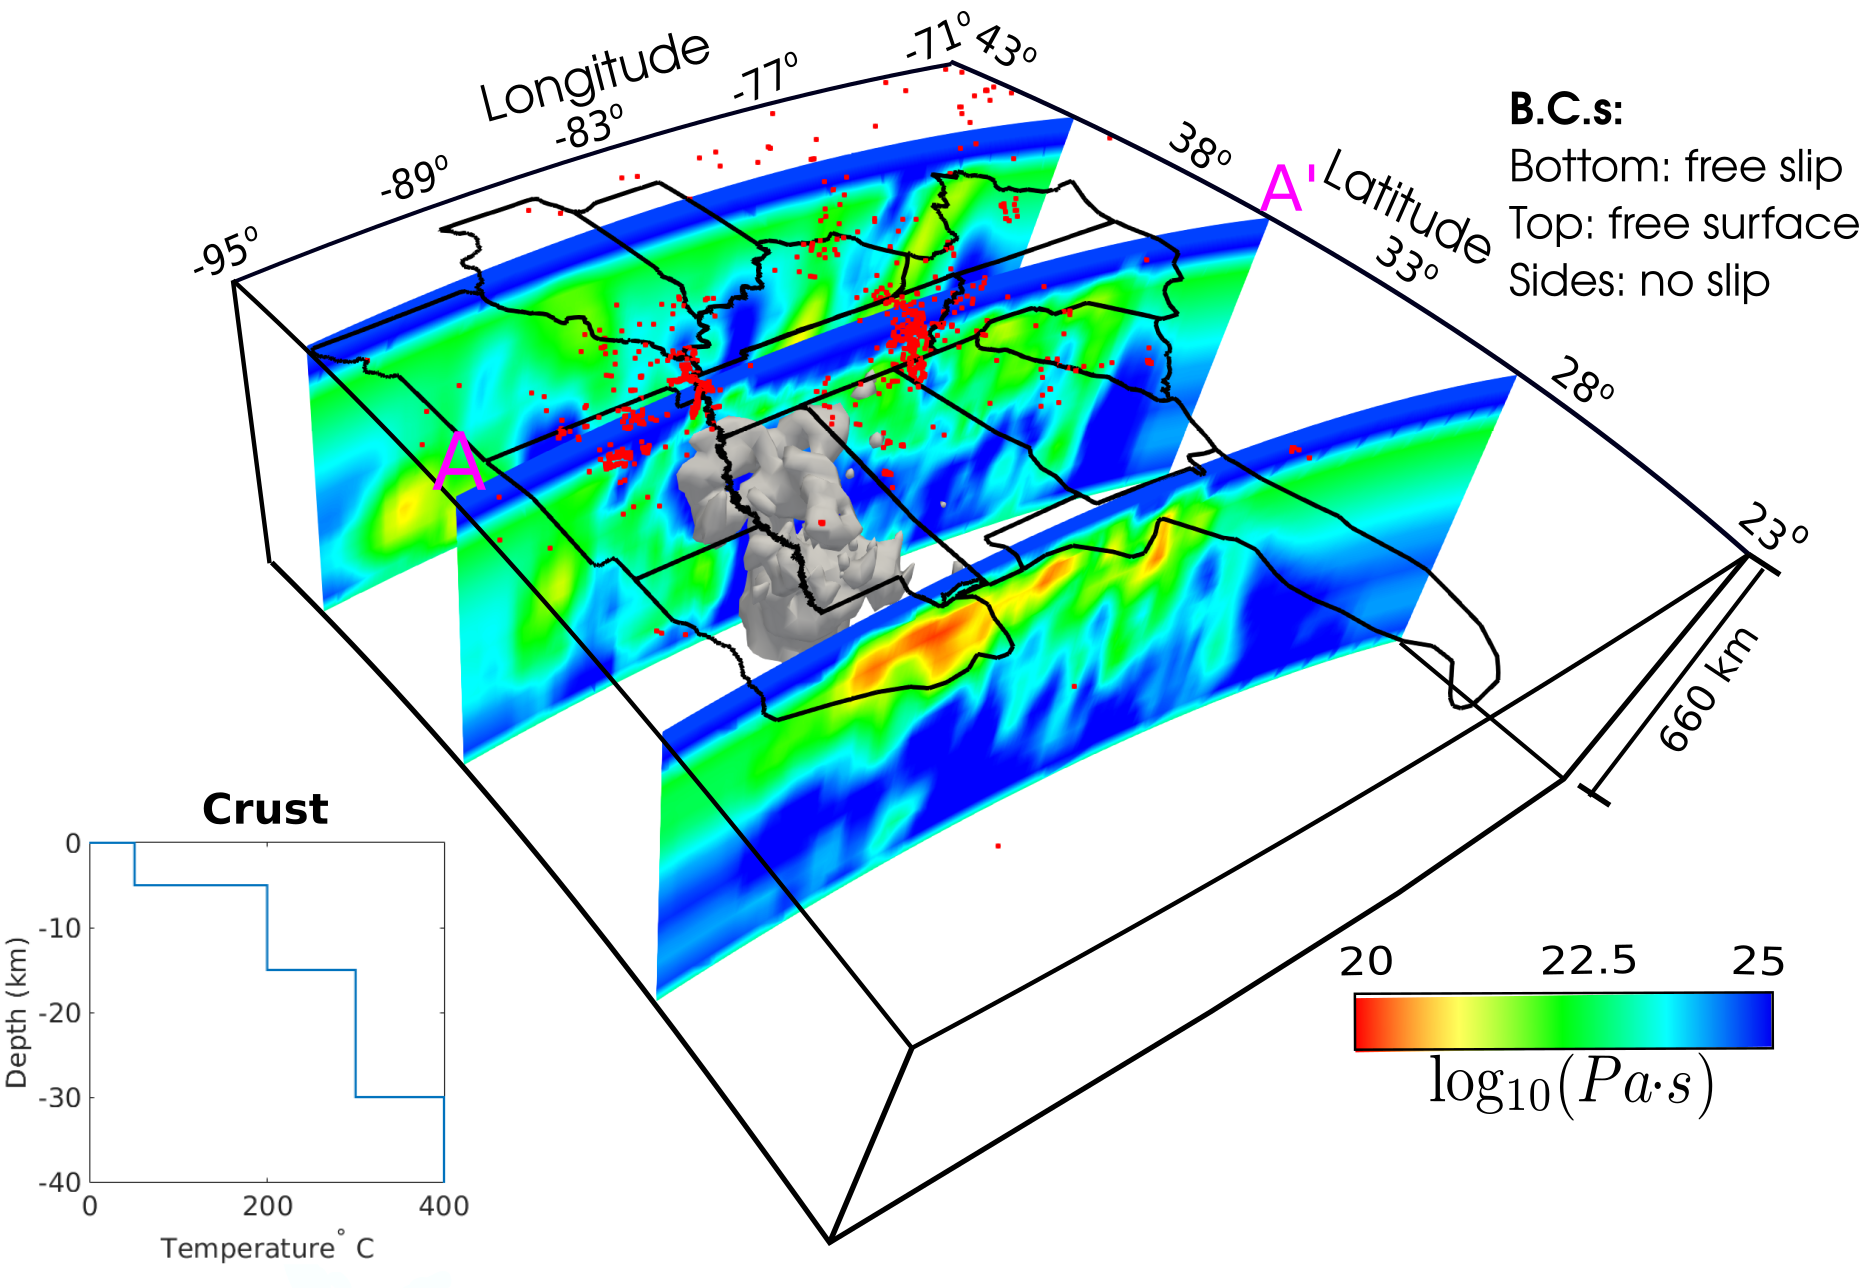
\includegraphics[width=0.75\linewidth]{figures/model_figure.png}
    \caption{Model setup with the computed rheology based on the regional tomography by \citet{Biryol_2016} and the boundary conditions applied. Gray isosurface represents P-wave anomaly $>$ 2 \% in the region proposed for lithospheric foundering. Instantaneous flow along slice AA' passing through the ETSZ and NMSZ is discussed in Fig. \ref{velocity_pattern}. Black lines indicate the state boundaries and red dots are the epicenters for the earthquake catalog used in Fig. \ref{figone}}.
    \label{fig_model}
 \end{figure}
    
    Upper mantle deformation is usually described by the combination of dislocation creep at lower temperatures than the melting temperatures of the rock and diffusion creep at high temperatures \citep{gordon1967thermally}. Our model employs both dislocation and diffusion creep with each type having different contributions depending on the temperature and pressure, such that the effective viscosity ($\eta_{eff}$) is computed as~\citep{billen2007rheologic}:
%
\begin{align}
    \eta_{\text{i}} &= \frac{1}{2} A^{-\frac{1}{n_i}} d^\frac{m_i}{n_i} \dot{\varepsilon_i}^{\frac{1-n_i}{n_i}} \exp\left(\frac{E_i + PV_i}{n_iRT}\right) \\
    \eta_{\text{eff}} &= \left(\frac{1}{\eta^\text{diff}} + \frac{1}{\eta^\text{dis}}\right)^{-1}
\end{align}

where $\eta^\text{diff}$ and $\eta^\text{dis}$ are viscosity due to diffusion and dislocation creep, respectively. $i$ corresponds to diffusion or dislocation creep, $A_i$ is the pre-exponential factor, $n_i$ is the power law exponent, $d$ is grain size taken constant as 5 mm (approximate value for olivine from \citet{karato1984grain} ), $m_i$ is the grain size exponent, $\dot{\varepsilon}$ is the second invariant of strain rate tensor, $R$ is the gas constant, $T$ is temperature obtained from the inversion of the P wave anomalies, $P$ is pressure, and $E_i$ and $V_i$ are the activation energy and volume respectively. The parameter values for diffusion and dislocation creep used to compute viscosity are given in Table \ref{table_model}.
%
\begin{table} \label{table_model}
    \caption{Values for dislocation diffusion creep$^a$}
    \centering
    \begin{tabular}{l c c c}
    \hline
     Parameter  & Symbol & Diffusion Creep & Dislocation Creep  \\
    \hline
      Pre-exponential factor & $A$ ($s^{-1}$) & $1.5e^{-16}$ & $0.3e^{-22}$   \\
      Power law exponent & $n$ & 1 & 3.5  \\
      Grain size exponent  & $m$ & 2 & 0   \\
      Activation energy  & $E$ (kJ/mol) & 300 & 530   \\
      Activation volume  & $V$ (cm$^3$/mol) & 6 & 20 \\
    \hline
    \multicolumn{2}{l}{$^{a}$ Values taken from \citet{karato1993rheology}.}
    \end{tabular}
\end{table}

Many studies have used a free-slip boundary at the 660-km discontinuity to mimic the restricted flow of material through it~\citep[e.g.,][]{arcay2007slab, billen2007rheologic, quinquis2011role}) and we adopt this free-slip bottom boundary (Fig. \ref{fig_model}) condition. For lateral boundaries, we tested our model with both free-slip and no-slip conditions and verified that the velocity fields at the seismic zones have the same pattern with up to 5\% magnitude difference. In this study, we only show the results for the no-slip conditions. We let the top boundary be a free surface
%I don't think you need explain this: based on \citet{kaus2010stabilization} free surface stabilization implemented in ASPECT) 
that can develop topography in response to the instantaneous flow in the mantle. We test a model with an additional lateral area of 5$^{\circ}$ by 5$^{\circ}$, surrounding our domain to check the results affected by the boundary conditions. The overall resultant velocity and stress field is similar with the current model domain but the magnitude at our depths of interest (15 km) near the boundaries is a smaller ( 10 - 15 \%) as the viscous effect of the same heterogeneity is now spread over a larger area. We show only the results for the smaller domain because the seismic zones are still sufficiently far from the model domain boundaries.

We calculate the static change in Coulomb stress using the equation \citep{king1994static}:
\begin{equation}
    \Delta C = \Delta \tau - \mu' \Delta \sigma_n,
\end{equation}
%
where $C$ is the Coulomb stress according to Coulomb failure function (CFF), $\tau$ (positive in the direction of slip). and $\sigma_n$ (positive when compressive) are the projected shear and normal stress for a particular fault orientation respectively, and $\mu'$ is the effective coefficient of friction after accounting for pore pressure. $\Delta$ represents the change between the two models for which CFF is calculated. Our model results are follows the right hand rule, such that the left-lateral and the normal motion is described by negative sign with $\tau$.
% High $\mu$ between 0.5 and 0.8 is associated with \annote[EC]{limited}{What do you mean?} fault cohesion and therefore, \annote[EC]{slip while lower values, i.e. 0-0.5 are generally taken for smooth sealed faults capable of larger slip accumulation}{The meaning of this sentence is not clear to me.} \citep{parsons1999stress}. 
Since we do not have sufficient constraints on the effective friction coefficients for the faults in the study area, we use a value of 0.6 based on \citet{hurd2012intraplate} and the observed repeated small-magnitude earthquakes ($M_w <$ 4.) in this region. 

We calculate the CFF at the approximate location of the seismic zones, ETSZ, SCSZ, CVSZ, GCSZ and the northeastern arm of the NMSZ (NMSZ\_NE), which are contained in the well-resolved region  in~\citet{Biryol_2016} tomography. CFF values are computed with respect to the optimal fault geometries based on the focal mechanism and earthquake relocation at 15 km depth for all the seismic zones. The zones and their optimal fault orientation is mentioned in Table \ref{table_fault}. 

% the ETSZ \citep{powell1994seismotectonic, cooley2015new, powell2016grenville}, GCSZ \citep{munsey1985focal}, NMSZ\_NE \citep{chiu1992imaging, shumway2008focal} and SCSZ \citep{madabhushi1993fault, hurd2012intraplate}. The mean optimal fault geometry from these studies are as follows: Strike N$10^\circ$E vertical right-lateral strike-slip faulting for GCSZ, NMSZ\_NE, ETSZ and some part of SCSZ, another set of vertical fault plane for ETSZ that is striking E-W left-lateral (ETSZ-2), Strike N$30^\circ$W right-lateral dipping 70$^\circ$ SE for CVSZ and N$30^\circ$W thrust fault dipping at $60^\circ$ SE for SCSZ. 


\begin{table}
\caption{Seismic Zones$^{*}$ and their associated optimal fault geometries}
\centering
\begin{tabular}{ c c c c } 
    \hline
    Seismic Zone & Strike, Dip & Sense of motion & Reference \\
    \hline
    NMSZ\_NE &  N$10^\circ$E, 90$^\circ$ & right-lateral & \citet{chiu1992imaging, shumway2008focal} \\ 
    \multirow{2}{2em} {ETSZ} & \multirow{2}{6em}{N$10^\circ$E, 90$^\circ$; E-W, 90$^\circ$} &  \multirow{2}{6em}{right-lateral; left-lateral} &  \multirow{2}{16em} {\citet{powell1994seismotectonic, cooley2015new, powell2016grenville}} \\ & & & \\
    GCSZ & N$10^\circ$E, 90$^\circ$ & right-lateral  & \citet{munsey1985focal} \\ 
    CVSZ & N$30^\circ$E, 50$^\circ$ SE & thrust  & \citet{wu2015aftershock}  \\ 
    SCSZ & N$30^\circ$W, 60$^\circ$ SE & thrust &  \citet{madabhushi1993fault, hurd2012intraplate}\\    
    \hline
\end{tabular}
 \begin{tablenotes}
    \begin {small}
        \item[1] $^{*}$ NMSZ\_NE: North eastern arm of New Madrid Seismic Zone; ETSZ: Eastern Tennessee Seismic Zone; GCSZ: Giles County Seismic Zone; CVSZ: Central Virginia Seismic Zone; SCSZ: South Carolina Seismic Zone.
     \end{small}
  \end{tablenotes}
\label{table_fault}
\end{table}

To isolate the effects of upper mantle ($>$ 200 km depth) heterogeneities, we compare results from models with and without the high-velocity feature considered as foundering lithosphere. Our tomography-based model is denoted by HT (heterogeneous) hereafter. We use two other models for comparison. One has laterally homogeneous temperature below 200 km depth and is denoted by HM. The other is identical with HT except that the high-density structure shown as the isosurface in Fig. \ref{fig_model} is removed and replaced with the reference values for the space enclosed by the isosurface. This model is denoted by HR.

%%%
\section{Model results}
We calculate changes in differential ($\Delta|\sigma_1 - \sigma_3|$) and Coulomb stress ($\Delta$ C) in HT relative to HM and HR, denoted by HT$-$HM, HT$-$HR respectively. HT$-$HM represents the stress contributions from the mantle heterogeneity deeper than 200 km, while HT$-$HR shows only the contribution of the high-velocity structure interpreted as the foundering root. 

Fig. \ref{model_results}(a) shows the computed change in differential stress for HT$-$HM (i.e., $\Delta|\sigma_1 - \sigma_3| = |\sigma_1 - \sigma_3|_{HT} - |\sigma_1 - \sigma_3|_{HM}$) at the seismogenic depth of 15 km for this region~\citep[e.g.,][]{mazzotti2010state}). Large positive values of $\Delta |\sigma_1 - \sigma_3|>15$ MPa are observed at the locations, $F_1$ and $F_2$.  The seismic zones, ETSZ, SCSZ, GCSZ, CVSZ and NMSZ are overall correlated with positive $\Delta |\sigma_1 - \sigma_3|$ in the range of 2 to 10 MPa (\ref{model_results}b). On the other hand, differential stress changes in HT$-$HR show only a small positive values of 1 to 2 MPa in the horseshoe-shaped region surrounding the root and including the ETSZ and NMSZ (\ref{model_results}b).
%
\begin{figure}[h!]
    \centering
    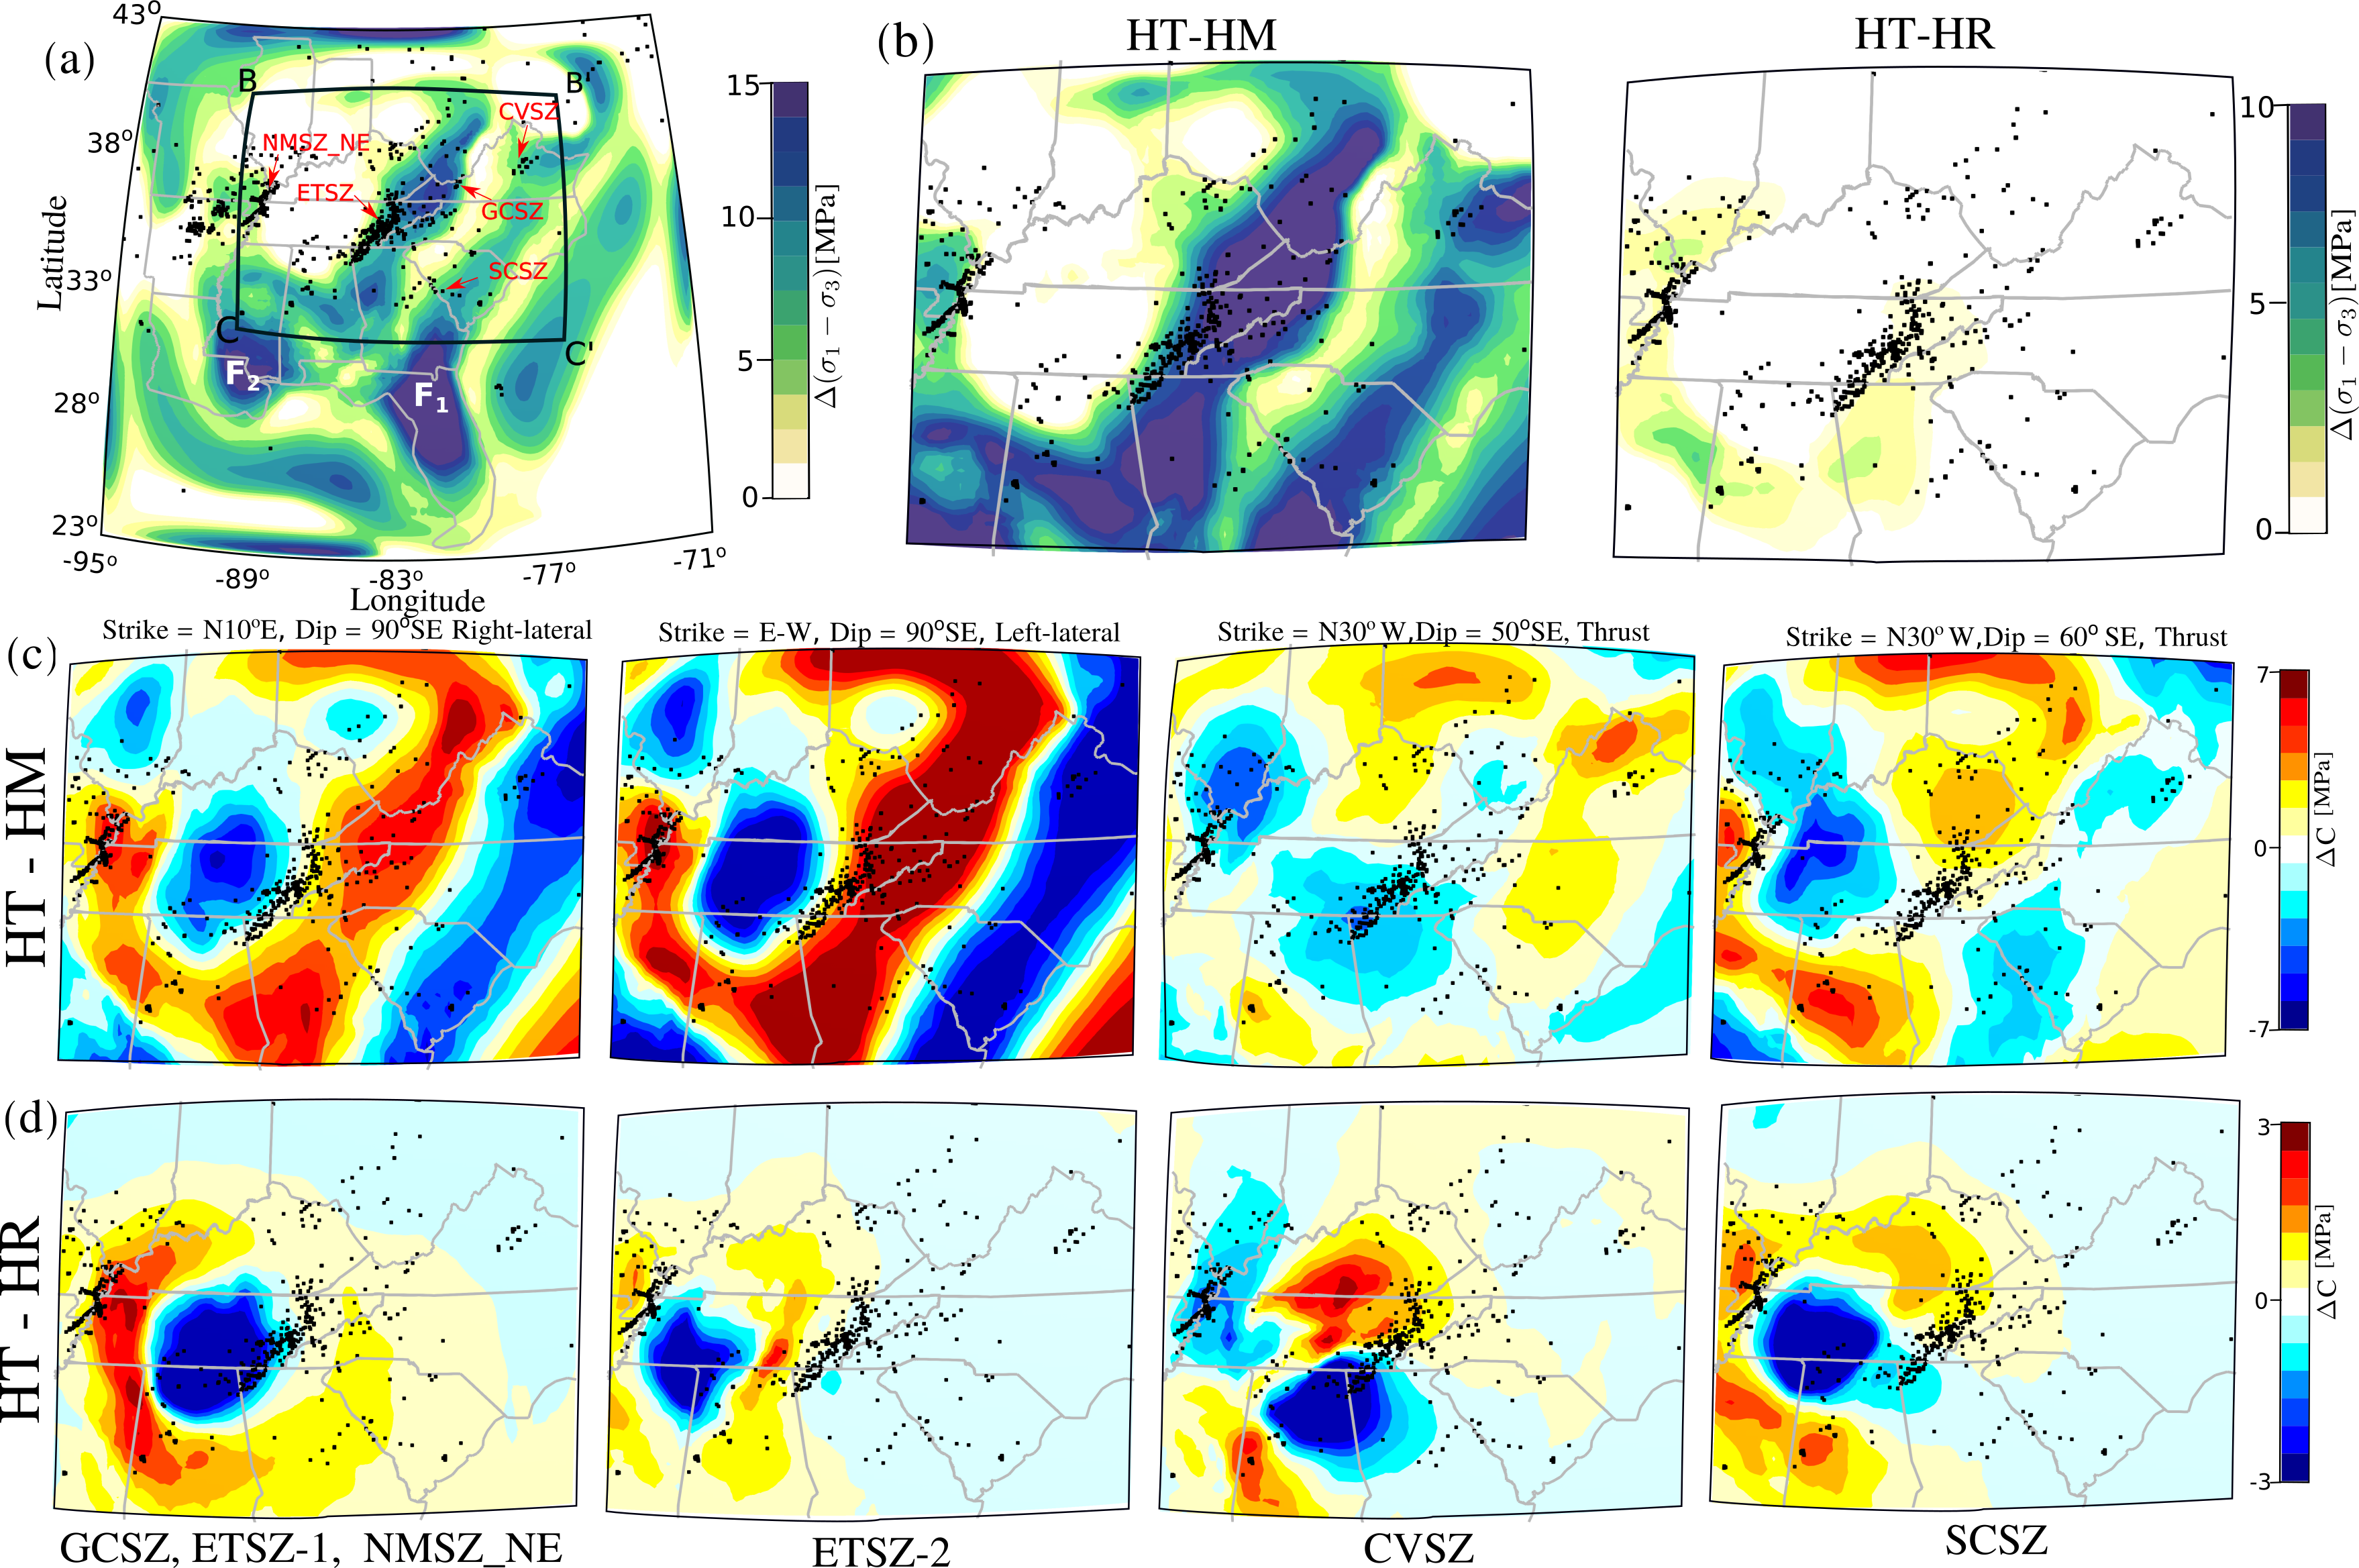
\includegraphics[width=\linewidth]{figures/model_results.png}
    \caption{Differential and Coulomb stress change derived from the tomography (HT) with two models: model homogeneous below 200 km depth (HM) and model with no root (HR). The root is marked as an isosurface in Fig. \ref{fig_model}. Data for earthquake epicenters, depicted by black dots, is from USGS data between 2011-2018. State boundaries are denoted by gray lines. Seismic zones investigated: North Eastern arm of New Madrid Seismic Zone (NMSZ\_NE), Eastern Tennessee Seismic Zone (ETSZ), South Carolina Seismic Zone (SCSZ), Giles County Seismic Zone (GCSZ) and Central Virginia Seismic Zone (CVSZ), are pointed in red. (a) Differential stress change between HT and HM at 15 km depth with a subset region BB'CC'. (b) Differential stress change of HT with HM (left) and HR (right) in BB'CC'. (c) Coulomb stress change of HT with HM for different fault orientations obtained by other studies involving the focal mechanisms and earthquake relocation. Seismic zone(s) and the corresponding fault geometry proposed for earthquakes in it is mentioned for each subplot. (d) Same as (c) but for Coulomb stress change of HT with HR. }
    \label{model_results}
\end{figure}

Coulomb stress changes ($\Delta $C) are computed for HT$-$HM (Fig.~\ref{model_results}c) and HT$-$HR (Fig.~\ref{model_results}d) at 15 km depth with respect to the optimal fault geometry in the five seismic zones, which are given in Table \ref{table_fault}. 
%The \annote[EC]{favorable}{Unify the terminology.} fault geometry along with the associated seismic zone(s) is mentioned for each subplot. 
%For a vertical fault orientated at N$10^\circ$E with right-lateral motion , 
Compared to the homogeneous HM model, the heterogeneous HT model produces a stress field that would increase the Coulomb stress in the GCSZ and  NMSZ\_NE by 4-5 MPa and by 1 MPa or less in the ETSZ with respect to the optimal fault orientation within these three seismic zones (Fig. \ref{model_results}c). For the vertical EW left-lateral faults, $\Delta$C$_{HT-HM}$ is as large as 5 MPa in most parts of the ETSZ. $\Delta$C$_{HT-HM}$ for faults with a strike of N$30^\circ$E and a dip of 50$^\circ$ SE with thrust motion shows only about 1-2 MPa increase in the CVSZ. The presence of the mantle heterogeneities does not increase the Coulomb stresses in the SCSZ relative to the homogenous model for optimally oriented faults in that seismic zone, which are thrust faults striking at N$30^\circ$W and dipping at $60^\circ$ SE. %, which is the  for shows not much correlation between the seismicity in SCSZ and positive $\Delta $C (Fig. \ref{model_results}(c)). 

Compared to the stress field without the foundering lithospheric root (HR), the stress field due to the root increases the Coulomb stress by up to 3 MPa in NMSZ\_NE for the seismic zone's optimal fault orientation (Fig. \ref{model_results}d). However, in the other seismic zones with the same optimal fault orientation, ETSZ and GCSZ, $\Delta $C$_{HT-HR}$ is weakly positive or even negative. The magnitude of $\Delta $C$_{HT-HR}$ is less than 1 MPa in ETSZ, CVSZ and SCSZ for their respective optimal fault orientations, indicating negligible effects of the root on those regions. 
    
    %%%%%
\section{Discussion and Summary}
%    In this study, we investigate the stress effects due to upper mantle heterogeneity, $>$ 200 km depth, and isolated lithospheric instability on the intraplate seismicity of the CEUS using numerical models based on the temperatures calculated from the \citet{Biryol_2016} tomography results. Many possible stress concentrators in the CEUS have been proposed to explain the seismicity \citep[e.g.,][]{levandowski2016dense, zhan2016stress} but analysis done here invoking deeper upper mantle structures and impact collectively on the seismicity in the CEUS has not been done before. 
    
    %We compute changes in differential stress and the Coulomb stress for particular fault orientations in the seismic zones: ETSZ, GCSZ, SCSZ, SCSZ and NMSZ (see Fig. \ref{figone} for their locations) due to both mantle heterogeneity and the lithospheric root in models HT$-$HM and HT$-$HR respectively. We observe 
    The foundering root appears to have an area of influence that includes only the ETSZ and NMSZ; the HT$-$HR case isolates the effects of the root and shows positive changes in differential stress magnitude only in the ETSZ and NMSZ\_NE. On the other hand, the HT$-$HM results involving the combined effects of all the mantle heterogeneities show that those mantle heterogeneities would increase differential stress relative to a hypothetical homogeneous mantle in all of the considered seismic zones (ETSZ, GCSZ, SCSZ, SCSZ and NMSZ\_NE). 
    
    %The Coulomb stress change is calculated at the selected fault orientations determined from previous studies on focal mechanism and earthquake hypocentral relocation in these seismic zones \citep[e.g.,][]{cooley2015new, powell2016grenville, munsey1985focal, chiu1992imaging}. In HT$-$HM, ETSZ, GCSZ and northeastern arm of NMSZ show an increase in Coulomb stress for the proposed fault orientation in these regions and CVSZ shows a weak positive increase while SCSZ overlies in the stress shadow, i.e. negative Coulomb stress change. Conversely, HT$-$HR does not show strong correlation between seismiciy and the Coulomb stress increase at all seismic zones except NMSZ.
    
     We quantify the optimal fault orientation for failure based only on our model results by calculating the Coulomb stress changes in the seismic zones for a wide range of fault geometries: strikes from N$30^\circ$W to N$90^\circ$E, dips from $10^\circ$ SE to $90^\circ$ SE % at intervals of $10^\circ$, for 
     for all the possible slip directions (right-lateral, left-lateral strike-slip, normal and thrust faulting). Results for HT$-$HM are shown in Fig. \ref{cs_ht_hm} and those for HT$-$HR in Fig. \ref{cs_ht_hr}. We restrict our fault orientations between E-W and NNW-SSE because the orientations of faults in this region are confined within these ranges according to previous studies~\citep{shumway2008focal, hurd2012intraplate, johnson2014earthquake, cooley2015new}. Since the effects of the root are spatially limited to the ETSZ and the NMSZ (Fig. \ref{cs_ht_hr}) and are smaller in magnitude compared to HT$-$HM (Fig. \ref{cs_ht_hm}), we identify the most optimally orientated fault plane as the orientation and sense of motion where $\Delta$C$_{HT-HM}$ is maximized.
 %    
\begin{figure}[ht]
    \centering
    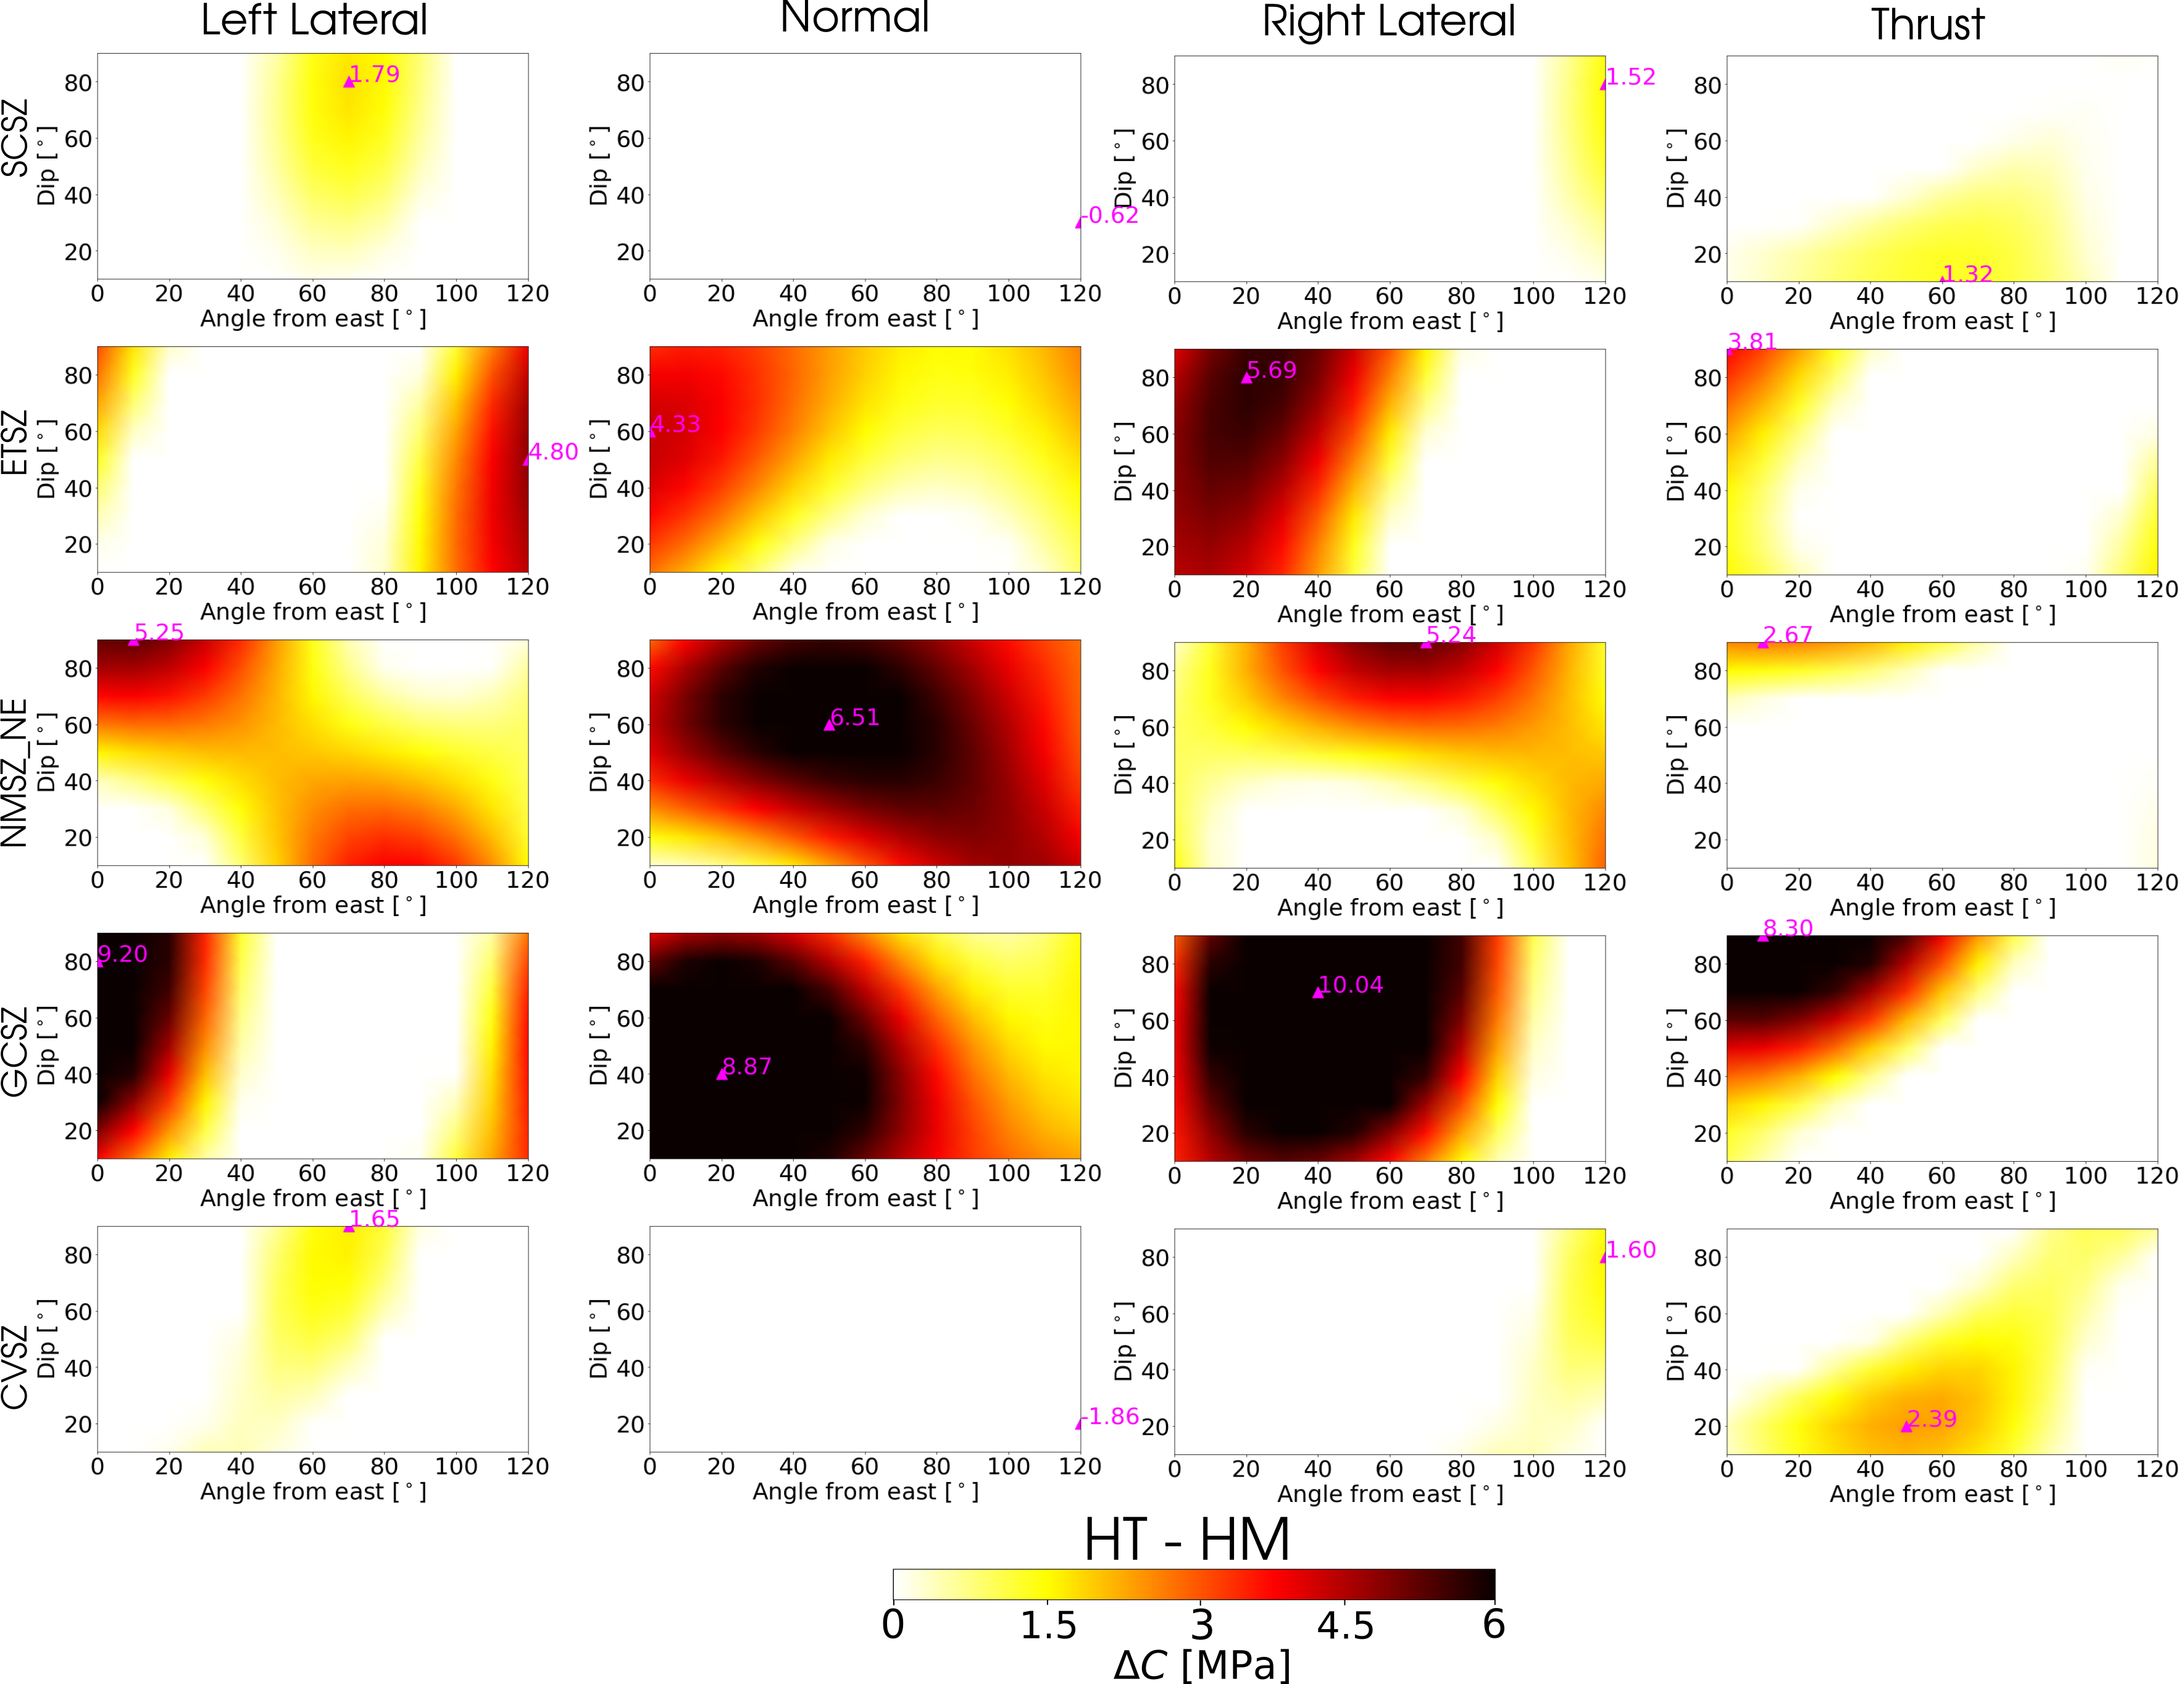
\includegraphics[width=\linewidth]{figures/ht_hm_summ.png}
    \caption{Coulomb stress change of HT with HM in seismic zones, CVSZ, ETSZ, SCSZ, GCSZ and North-Eastern segment of NMSZ (NMSZ\_NE) from $0^\circ$ to $120^\circ$ from East and dips from $10^\circ$ SE to $90^\circ$ SE at intervals of $10^\circ$, for all possible slip directions: right-lateral, left-lateral strike-slip, normal and thrust faulting. Subplots are also labeled with maximum $\Delta C$ and the orientation and dip where it occurs is denoted with a triangular marker.}
    \label{cs_ht_hm}
\end{figure}
%
\begin{figure}[ht]
    \centering
    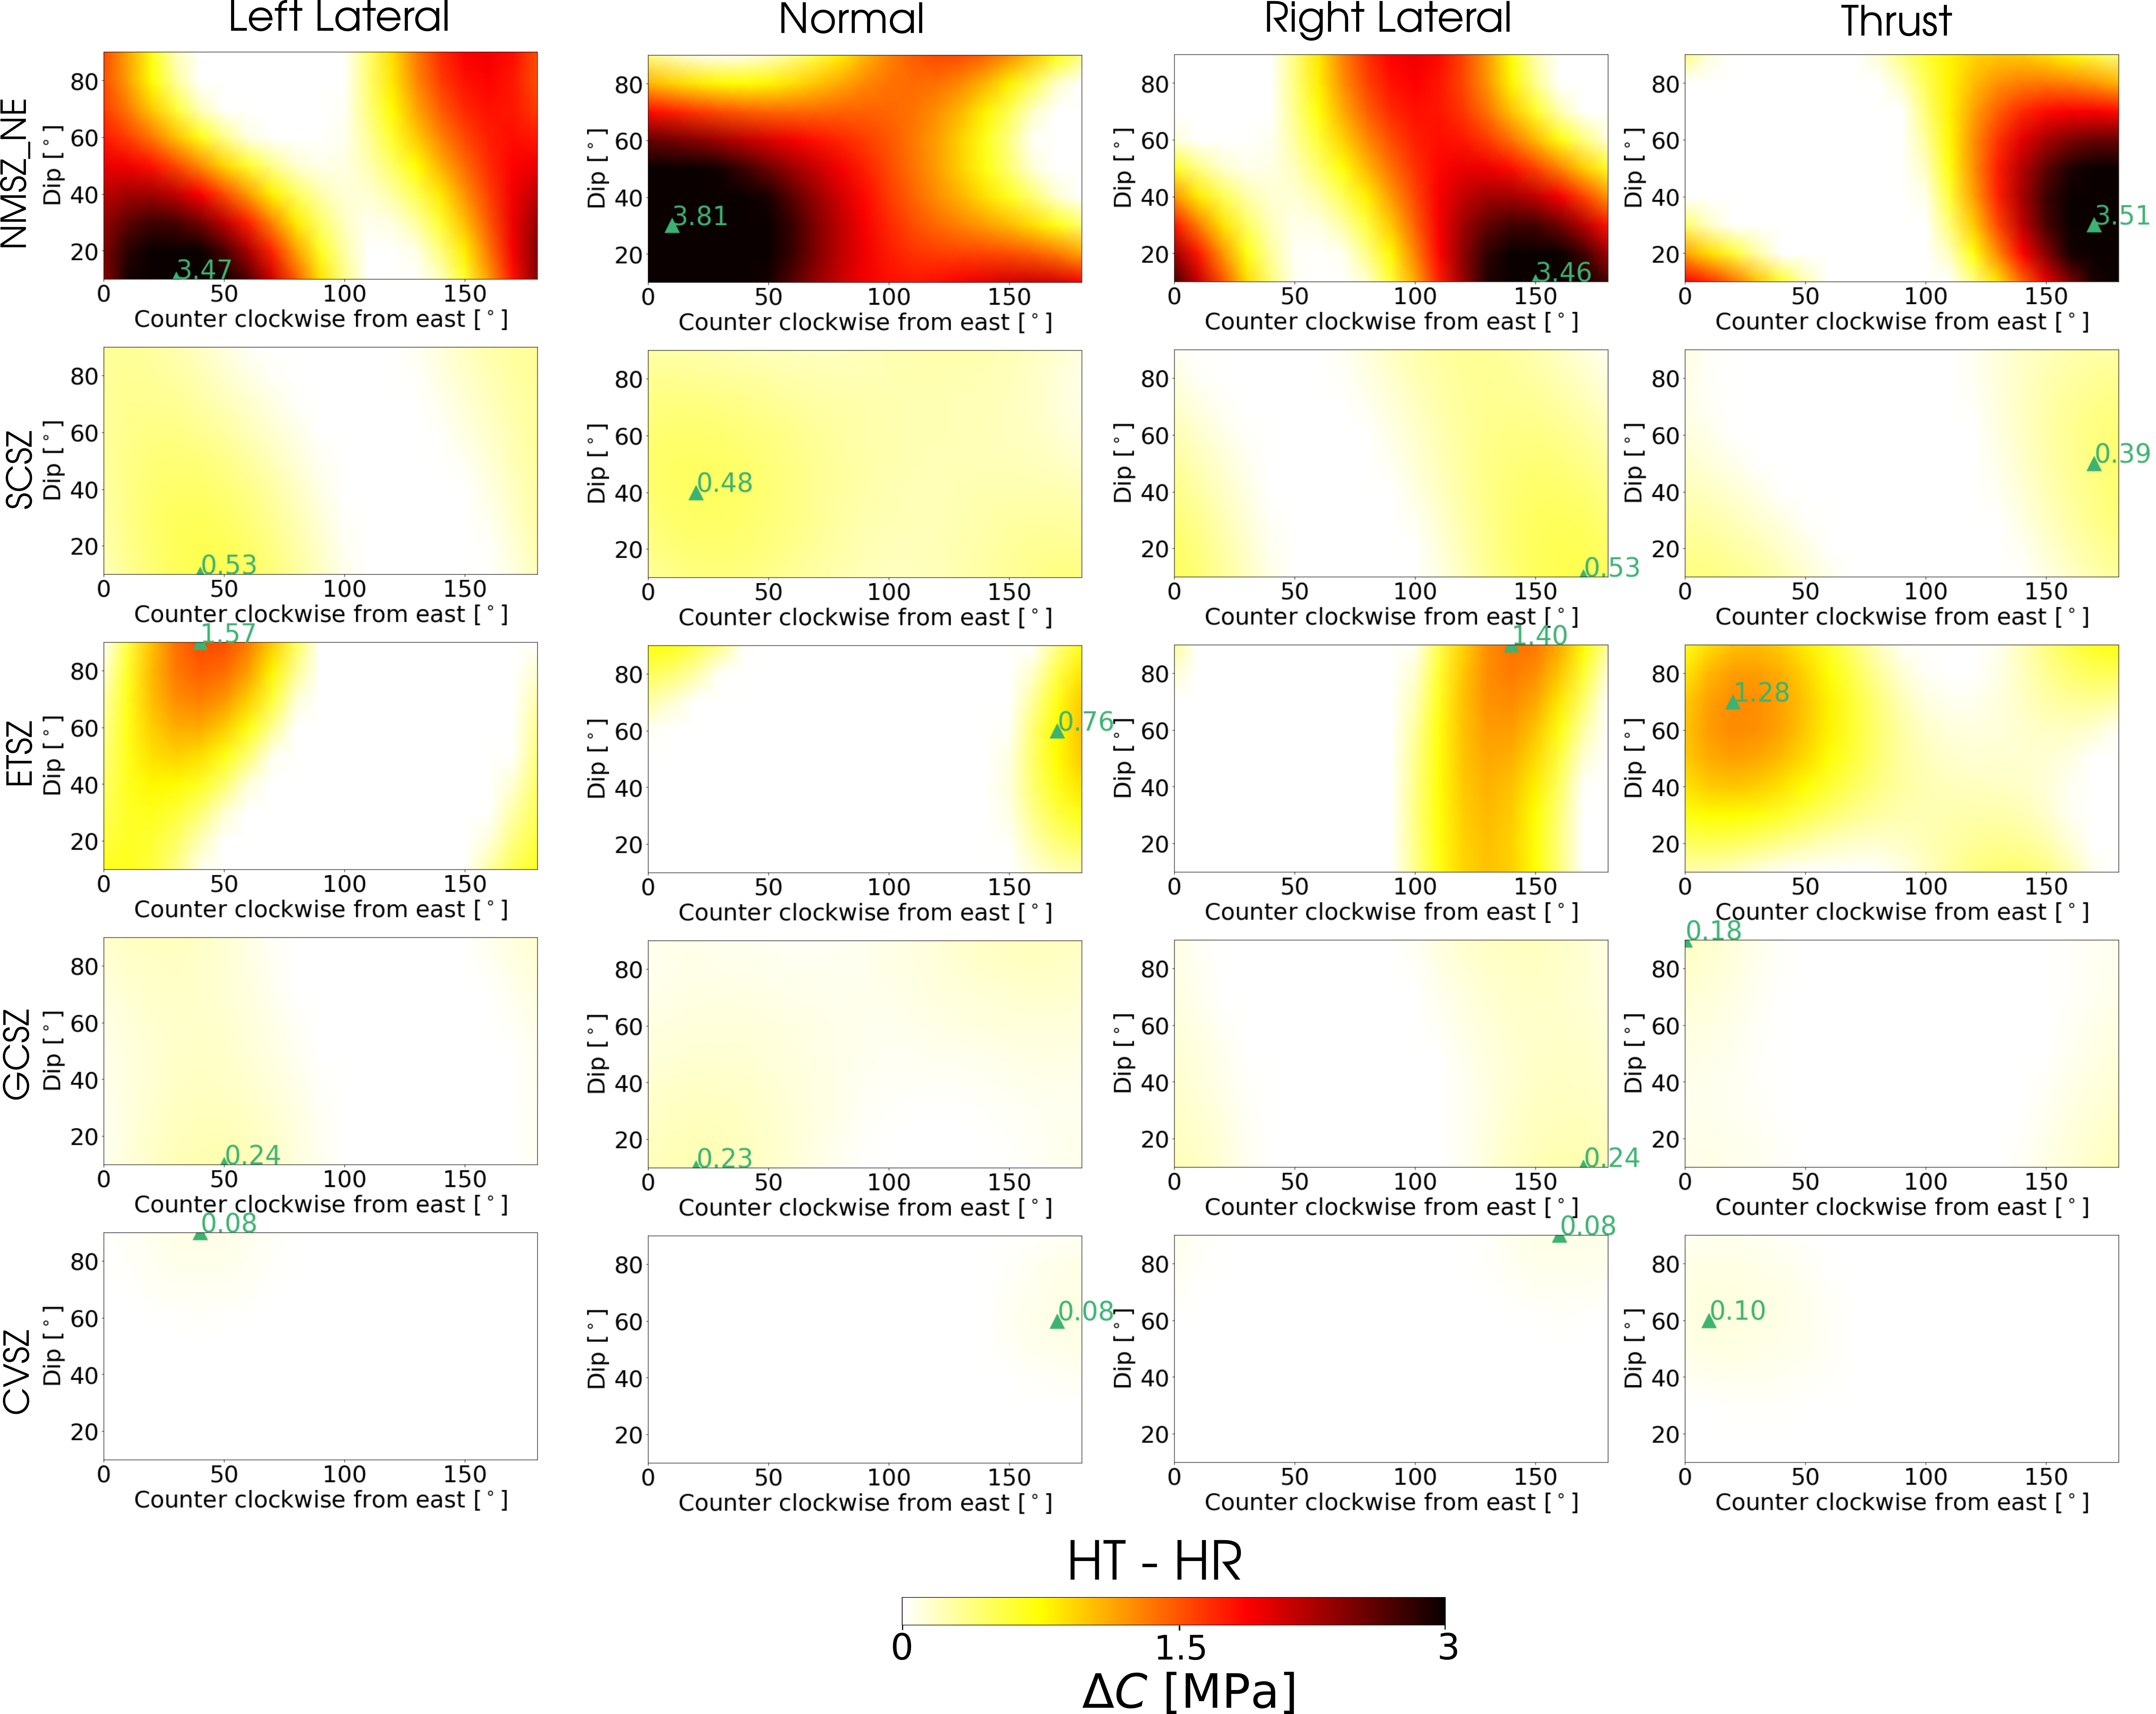
\includegraphics[width=\linewidth]{figures/ht_hr_summ.png}
    \caption{Same as in Fig. \ref{cs_ht_hm} but for change of HT with HR.}
    \label{cs_ht_hr}
\end{figure}

     The most optimally oriented fault planes in Fig. \ref{cs_ht_hm} based on our model results do not coincide with the proposed fault focal mechanism solutions in these seismic zones. There must be a number of reasons for the mismatch. Firstly, the presence of deeper ($>$ 200 km) mantle heterogeneity is not the only contributing factor for stress concentration in the CEUS. Other factors such as a dense sinking body in a weak lower crust as proposed by \citet{Pollitz_2001} or weak lower crust embedded in elastic lithosphere by \citet{Kenner_2000a} or glacial isostatic response from deglaciation of Laurentia by ~\citet{Grollimund_2001}, may also play a role at a shallow depth scale.  Secondly, most of the earthquakes in the CEUS occur at depths $<$ 20 km~\citep[e.g.,][]{bollinger1985seismicity, chiu1992imaging, powell2016grenville} on the reactivated faults formed from one or two episodes of Wilson cycles~\citep{thomas2006tectonic, wolin2012mineral}. The mantle tomography model in our study does not provide constraints on the geometry and strength of the shallow seismogenic faults created in the past. Thirdly, our model does not account for any tectonic stresses and only focuses on the local stress perturbations from the upper mantle. In reality, the presence of plate motion, as included by~\citet{zhan2016stress} \citet{levandowski2016dense}, may alter the stresses from heterogeneity. All these factors together or alone could change results for all or any of the seismic zone.
    
\begin{figure}[ht]
    \centering
    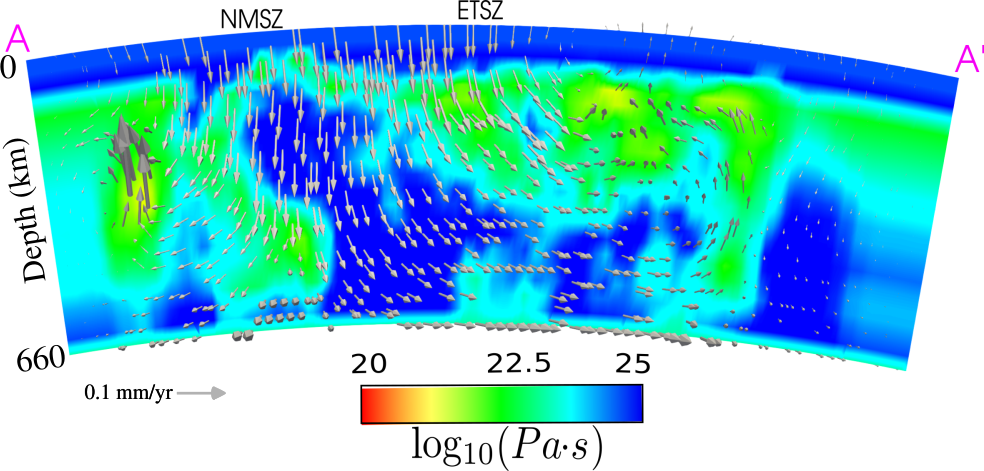
\includegraphics[width=0.9\linewidth]{figures/velocity_pattern.png}
    \caption{Velocity field at slice AA' (marked in Fig \ref{fig_model}) overlying the viscosity distribution computed from the temperatures based on the tomography by \citet{Biryol_2016}. High velocity vectors observed west of the NMSZ is from the upward return flow due to the downward pull of the lithospheric root and is likely an artifact due to fixed boundary conditions at the sides.}
    \label{velocity_pattern}
\end{figure}

    The stresses in our model arise from the instantaneous flow due to the upper mantle heterogeneity. Fig. \ref{velocity_pattern} shows the velocity field at slice AA$^{\prime}$ (marked in Fig \ref{fig_model}) in the model HT due to heterogeneous density computed from temperatures based on the tomography by \citet{Biryol_2016}. The region below both the NMSZ and ETSZ shows a downward velocity pattern and the upwellings induced from it are concentrated along the edges of the model domain. The upwellings are observed at the surface as features F$_1$ and F$_2$ marked in Fig.~\ref{model_results}. The downward flow pattern beneath the NMSZ due to the lithospheric root is opposite to the asthenospheric upwelling proposed by \citet{Biryol_2016}. However, this interpretation of the velocity field from our model depends on various parameters including viscosity of the asthenosphere and boundary conditions of the model. %We computed mantle viscosity solely based on the seismic tomography constraints and the actual value in the earth would be different. 
    Lower viscosity in the asthenosphere would reduce the lateral extent of the convection from the lithospheric root such that the surrounding NMSZ is not affected by the downward pull. However, even with lower viscosity of the asthenosphere it is still unlikely that the localized low-velocity anomaly below NMSZ would counteract the downward pull from the much larger positive anomaly lithospheric root. 
%    

\begin{figure}[h!]
    \centering
    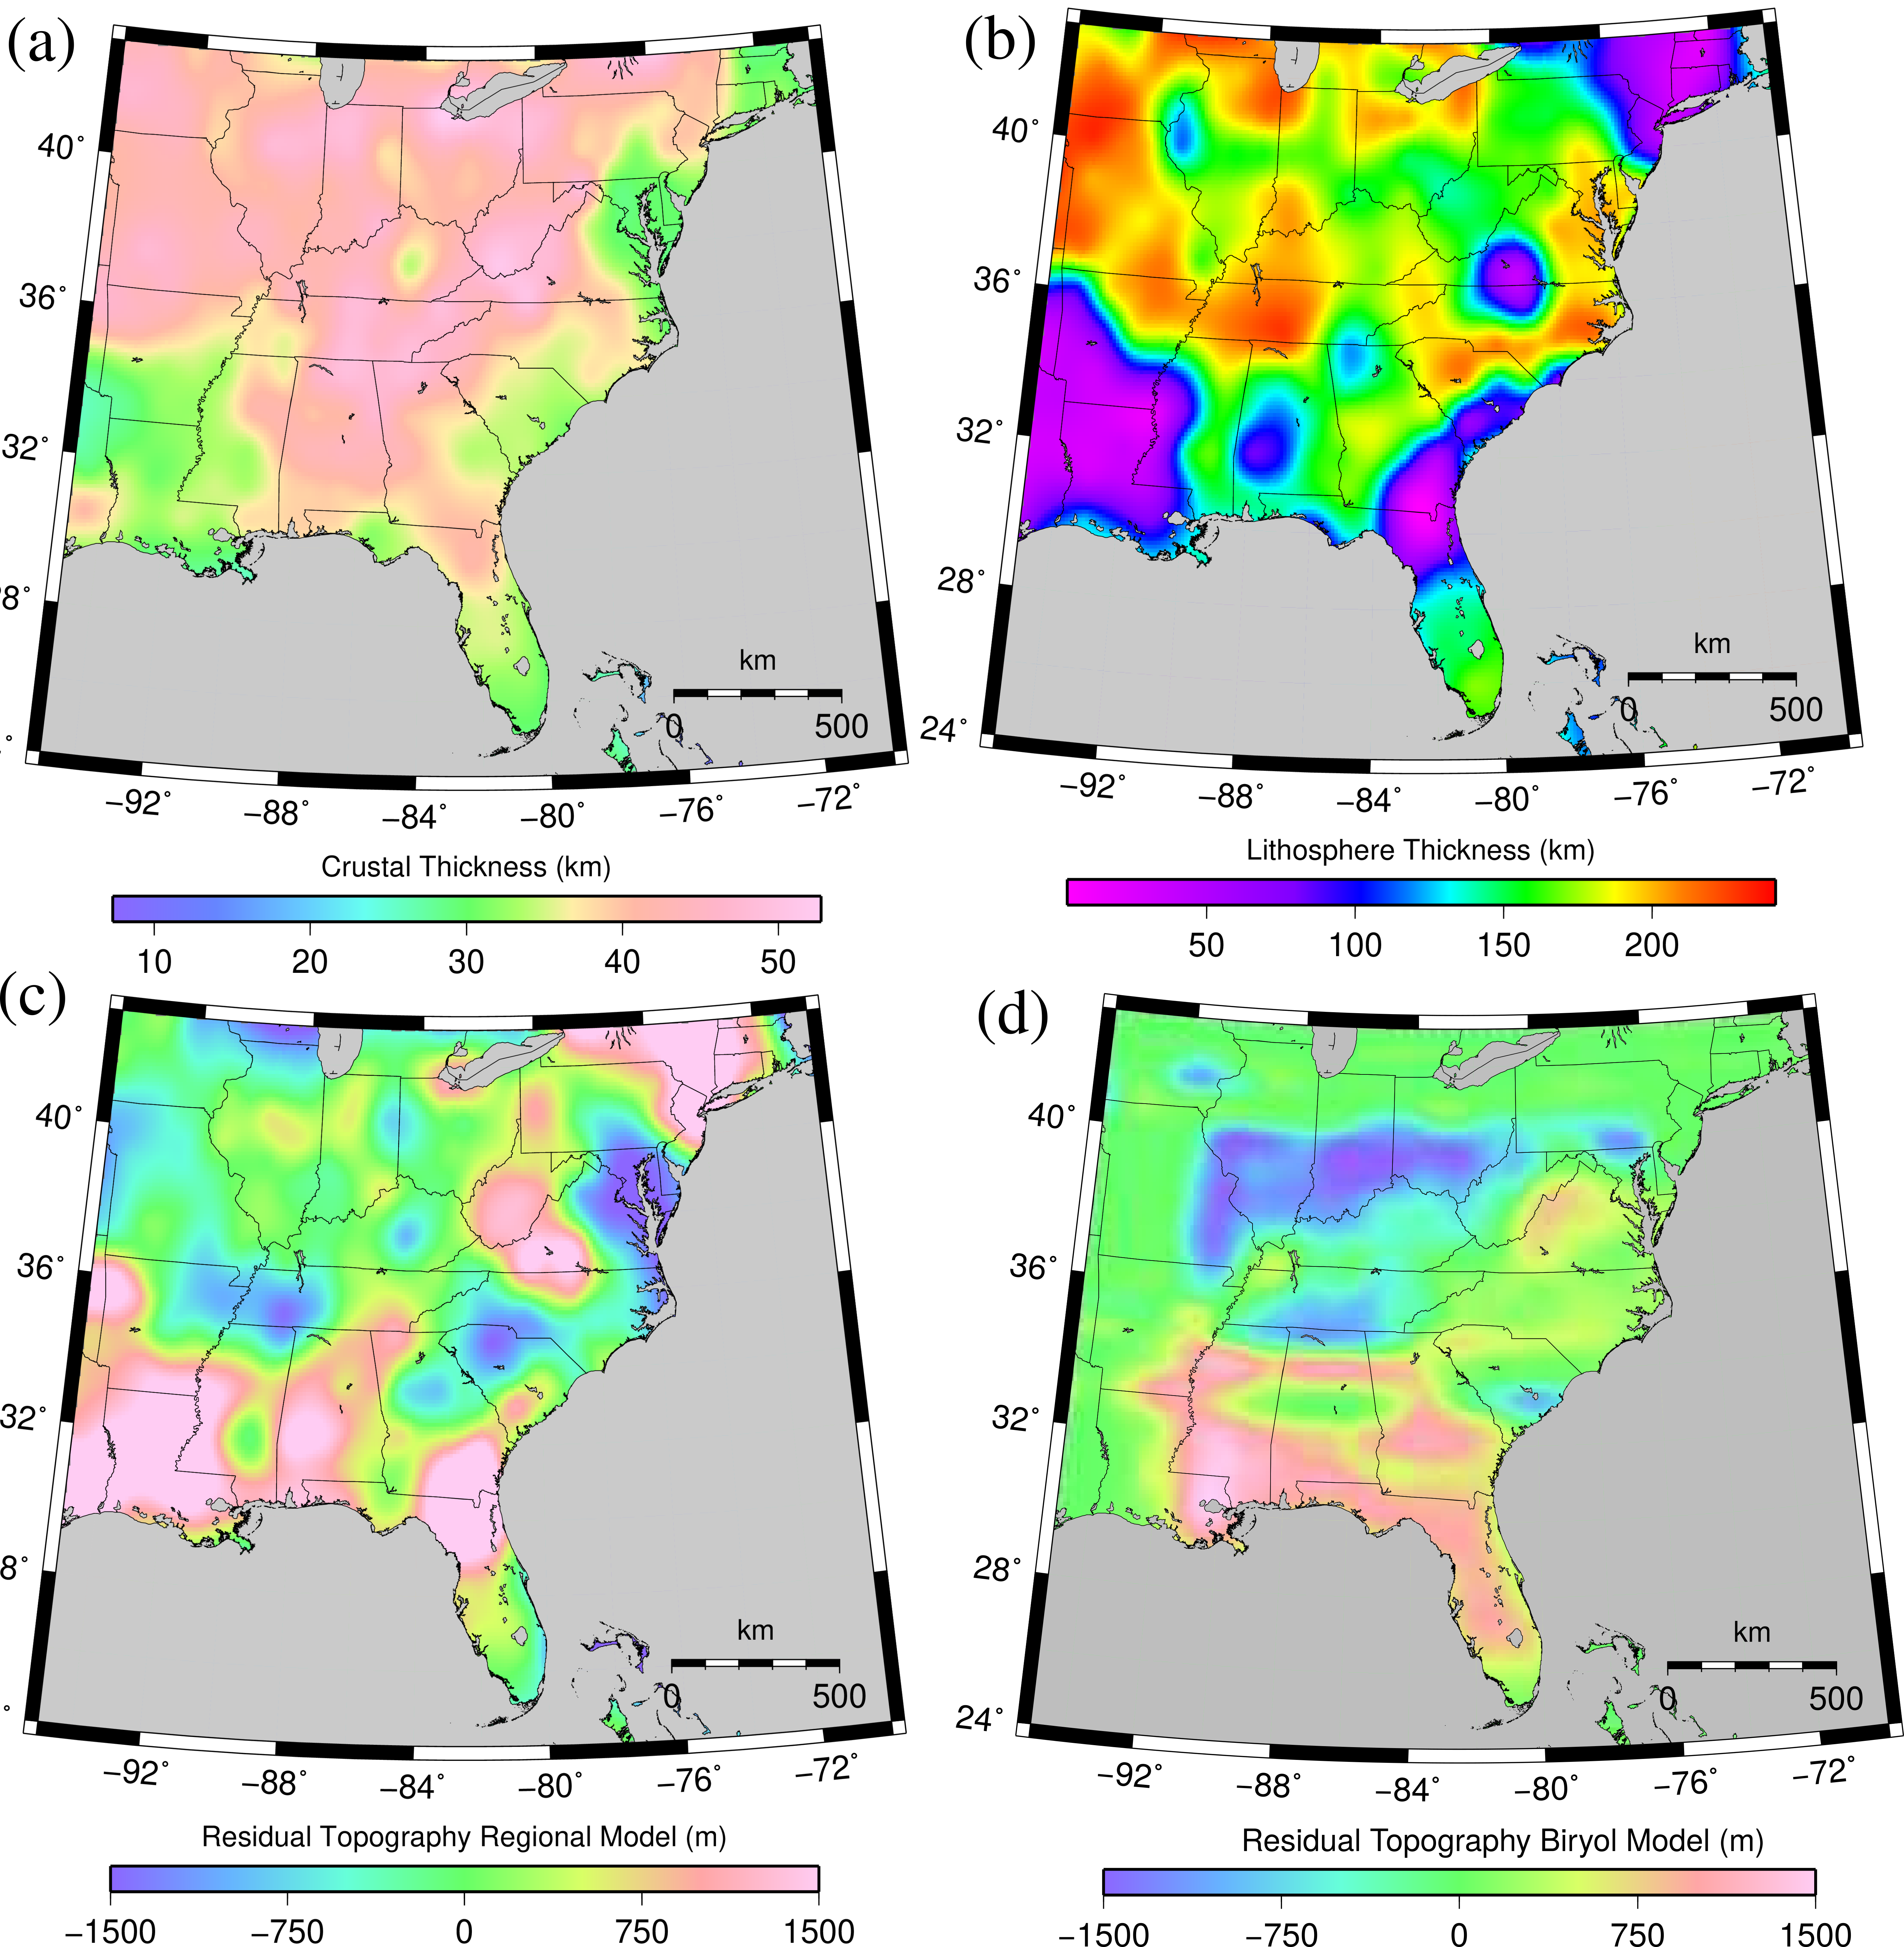
\includegraphics[width=\linewidth]{figures/topography.png}
    \caption{Residual topography calculated from densities based on the regional tomography by \citet{Biryol_2016} used in this study and from global models. (a) Crustal thickness from CRUST1.0 \citep{laske2013update}. (b) Lithospheric thickness from LITHO1.0~\citep{pasyanos2014litho1} (c) Residual topography calculated using (a) and (b). (d) Residual topography based on the temperatures calculated using the regional tomography used in this study. }
    \label{topo_res}
\end{figure}


% \note[EC]{What is the topographic relief in the study area? It must not be as large as $\pm$2000 m. If so, I'm not sure if it's reasonable that the residual topo has a greater relief than the surface... Maybe but what would be the meaning...?}
    We examine the topography generated due to the mantle flow generated from the upper mantle heterogeneity in Fig. \ref{topo_res}. We calculated residual topography in our study region following the approach by \citet{becker2014static} on the static and dynamic topography for the western US. We first calculate the isostatic topography. We use CRUST1.0~\citep{laske2013update} for crustal thickness and density (Fig. \ref{topo_res} a) and LITHO1.0~\citep{pasyanos2014litho1} for lithospheric thickness variations (Fig. \ref{topo_res}b). We assume a constant lithospheric density of 3300 kg/m$^3$ and a constant asthenosphere density of 3250 kg/m$^3$. These values are reasonable for a density contrast between the lithosphere and asthenosphere~\citep[e.g.,][]{bonnardot2008numerical, ito2011probing}. Although the crustal contribution to the topography is 2.25 times more dominant than the lithosphere for these density values, the residual topography is dominated by the lithospheric variations (Fig. \ref{topo_res}c) which are up to 8 times greater than the crustal thickness variations. We also calculate the residual topography from the mantle flow in our models due to the density distribution based on the \citet{Biryol_2016}s tomography results (Fig. \ref{topo_res}d). The discrepancy between the topography calculated using global crustal and lithosphere models and that based on the regional seismic tomography is expected. Firstly, the seismic tomography puts no constraints on the crustal structure and the crust is assumed to have a uniform thickness of 40 km to calculate the isostatic response, contrary to the crustal thickness and density variations obtained from the CRUST1.0 model. Secondly, the LITHO1.0 model is about 8 times coarser in resolution than the tomography study and we assume a constant density of 3300 kg/m$^3$ instead of the density based on the heterogeneous temperature. We therefore suggest that additional investigation into the accurate crustal and lithospheric thickness and density variation is required to observe any topography response from the upper mantle flow, which is not done in this study.
%

    
    We discuss the stress implications of lithospheric foundering using instantaneous models with a root but to address the mechanism for the origin of a lithospheric root in the CEUS, time-dependent modeling will be needed. Such investigation in this region would call for more sophisticated techniques such as backward advection modeling~\citep[e.g.,][]{conrad2003seismic}, quasi-reversibility~\citep{glivsovic2016new}, or adjoint methods~\citep[e.g.,][]{bunge2003mantle, liu2008reconstructing} for calculation of initial conditions on temperature, viscosity and density, which has not been done in this study. It has been proposed by \citep{Biryol_2016} that the lithospheric foundering could have started due to Rayleigh-Taylor instability beginning from the presence of an ecologized root as proposed by \citet{le2006mantle} in the western US. It is also possible that the dense high velocity mantle feature is part of the subducted Farallon slab below this region~\citep{schmandt2010seismic}. We do not comment on the origin of this high velocity feature but follow the naming convention by \citet{Biryol_2016} as a root in this study. Additional observations such as low dynamic topography at the surface would be required to confirm if the high velocity is indeed attached to the lithosphere or part of a remnant Farallon slab.
    
    In summary, based on the numerical model with heterogeneous temperature, density and viscosity based on the tomography by \citet{Biryol_2016}, we observe differential stress concentration due to the upper mantle heterogeneity at the major seismic zones in the CEUS: ETSZ, NMSZ, GCSZ, CVSZ and parts of SCSZ. We also examine the isolated effect of a positive P wave anomaly interpreted by \citet{Biryol_2016} as a lithospheric root and observe increased differential stress in the seismic zones surrounding the root (ETSZ and NMSZ). Coulomb stress was also increased in seismic zones ETSZ, GCSZ, NMSZ and CVSZ at their optimal fault orientations obtained from other studies when all the upper mantle heterogeneity is considered. Therefore, our results provide a possible mechanism for reactivation of the faults in the intraplate seismicity of the CEUS. This in turn helps to better associate seismic hazard with the seismic zones in the CEUS.
    
\appendix
\section{Appendix}

\begin{figure}[ht]
    \centering
    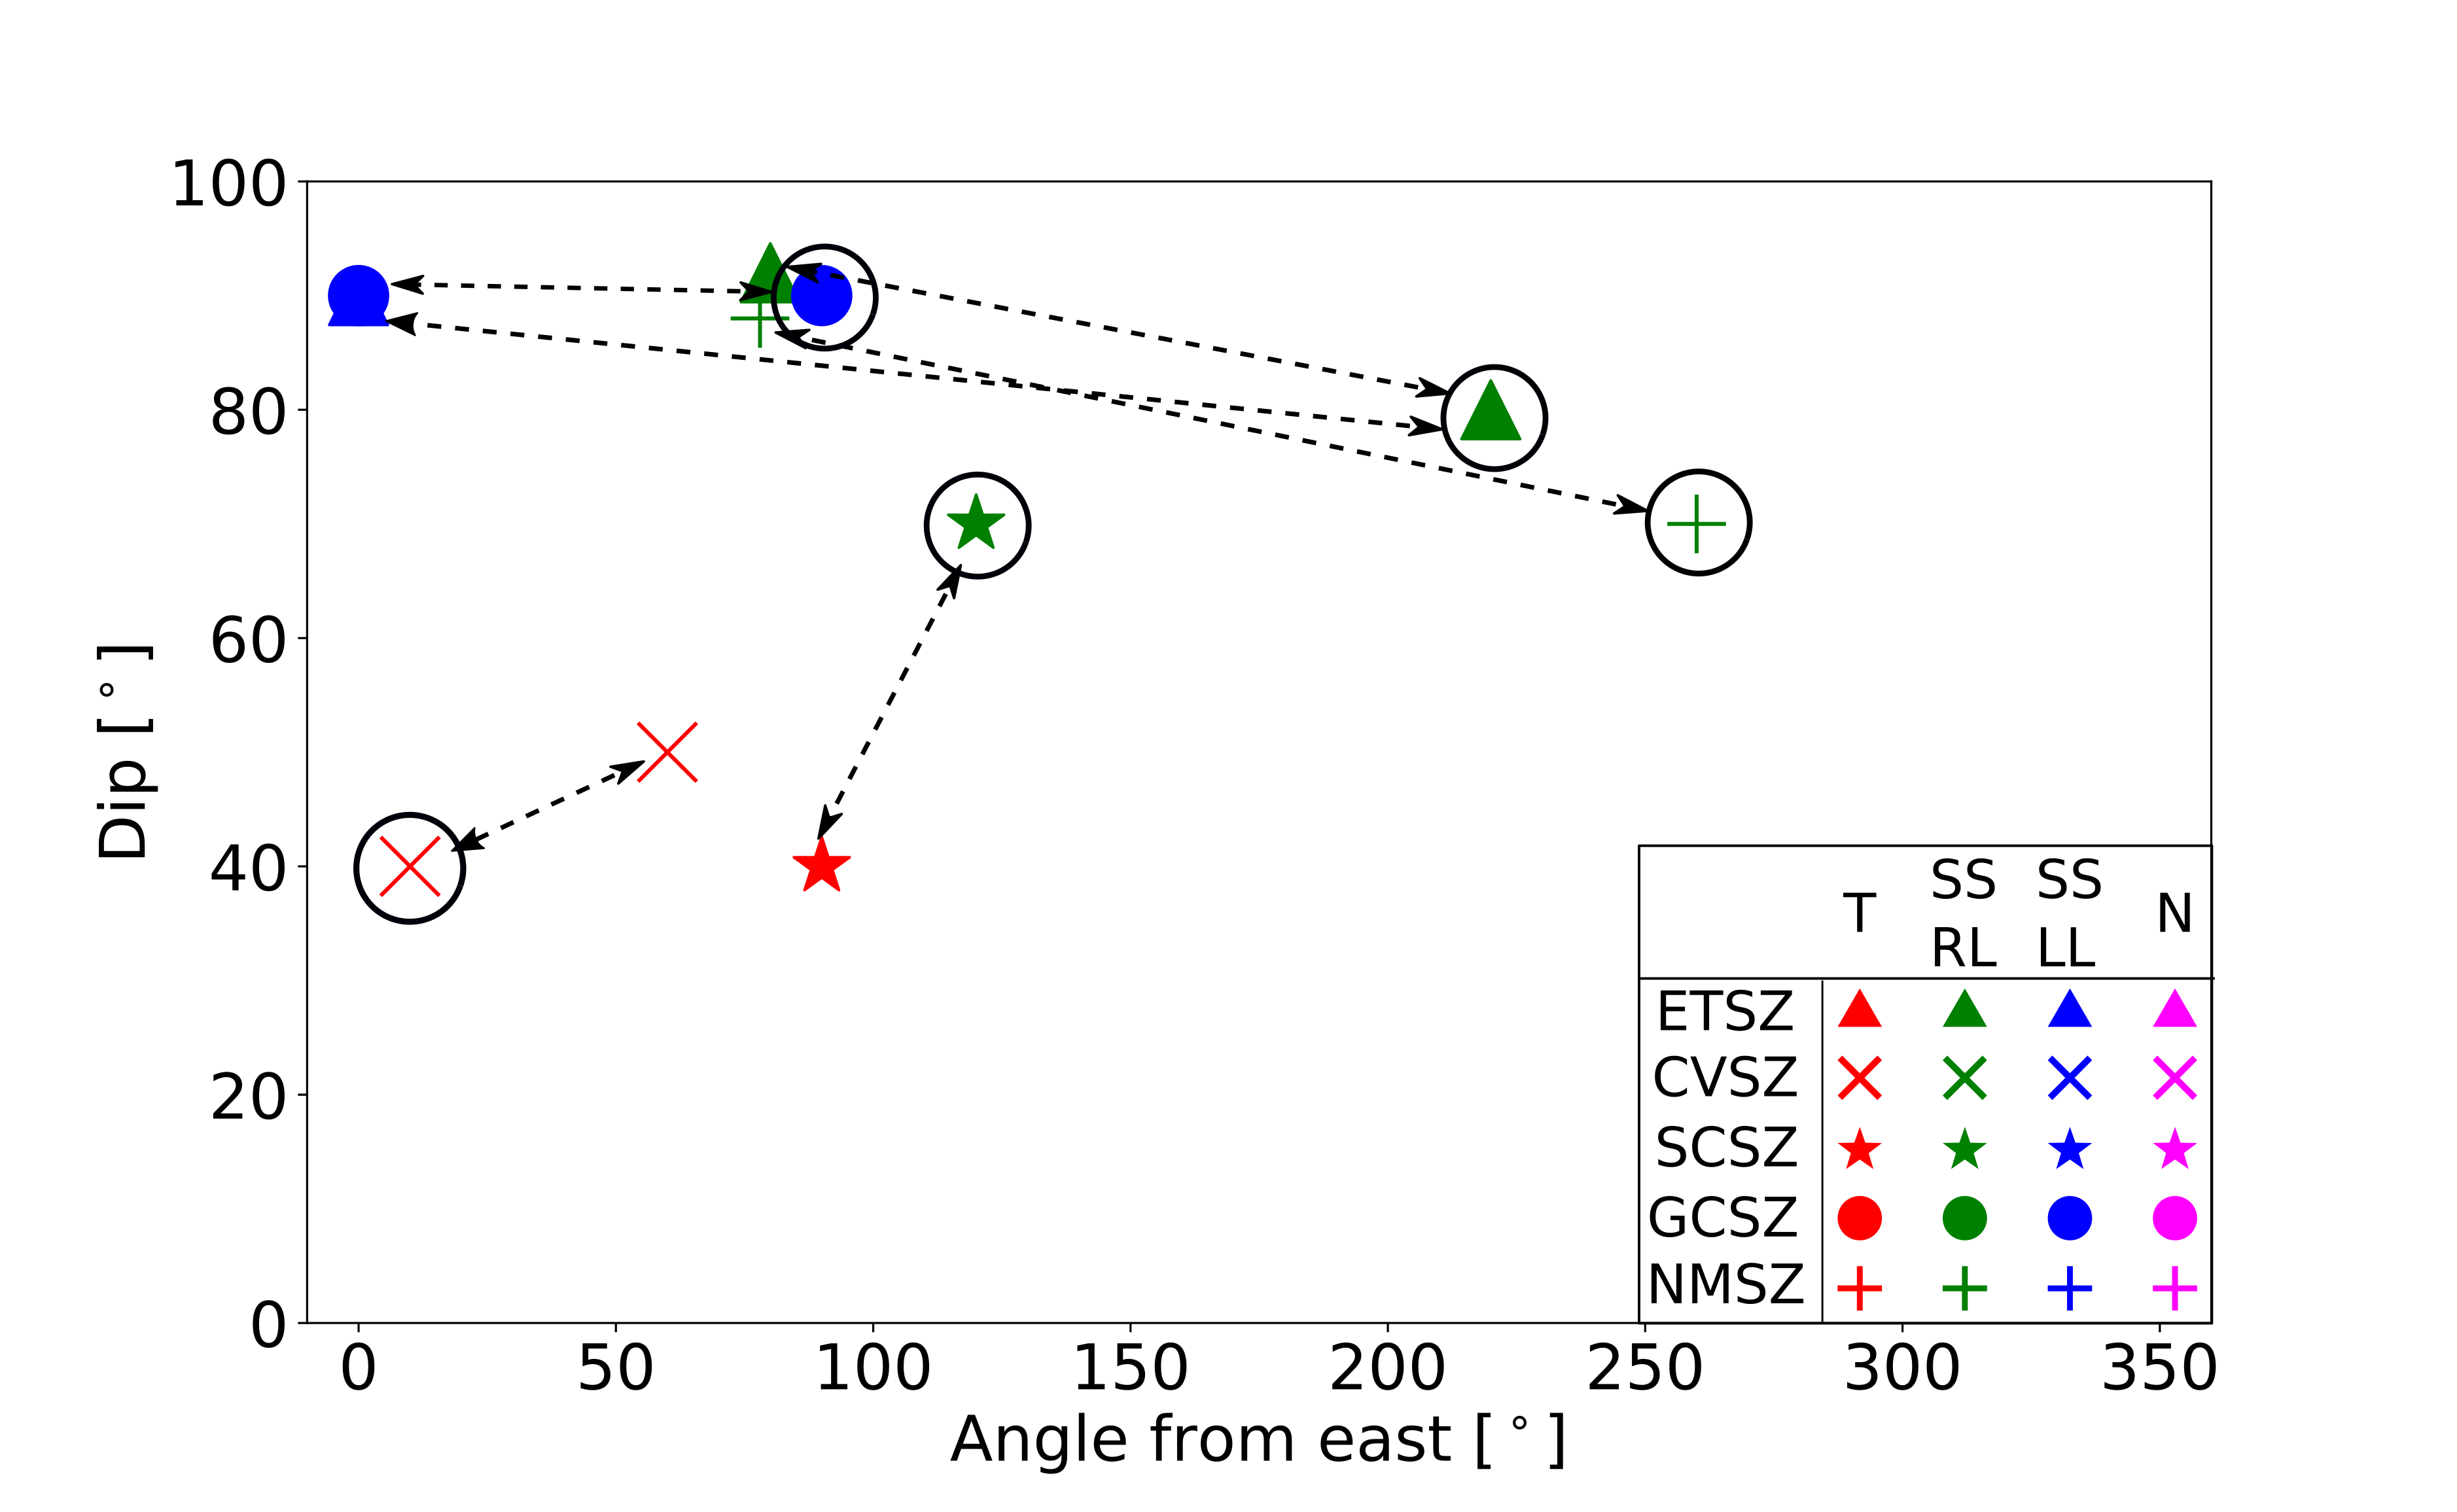
\includegraphics[width=0.8\linewidth]{figures/summ_stress.png}
    \caption{Proposed fault planes from other studies on focal mechanism and earthquake hypocenters and fault planes at which $\Delta$C$_{HT-HM}$ is maximum. The markers represent each of the seimic zones: New Madrid Seismic Zone (NMSZ), Eastern Tennessse Seismic Zone (ETSZ) South Carolina Seismic Zone (SCSZ), Giles County Seismic Zone (GCSZ) and Central Virginia Seismic Zone (CVSZ). The sense of fault slip is indicated with the color of the marker as thrust(T), right-lateral strike-slip (SS, RL), left-lateral strike slip (SS, LL) and normal (N). 'M' denoted near the marker represents the orientation at which $\Delta$C$_{HT-HM}$ is maximum in the model.}
    \label{summary}
\end{figure}


\begin{table}
\caption{Mineral physics data used in this study \tnote{1}}
\centering
\begin{tabular}{ l c c c c c c c c c } 
\hline
 \multirow{2}{3em}{Mineral} & \multirow{2}{3em}{Density ($kg/m^3$)} & \multirow{2}{3em}{$K_S$ (GPa)} & \multirow{2}{3em}{$\mu$  (GPa)}  & $K'$ & $\mu'$ &  \multirow{2}{4em}{$\partial K/\partial T$ (GPa/K)}  & \multirow{2}{4em}{$\partial \mu/\partial T$ (GPa/K)} & \multirow{2}{4em}{$a_0 (10^{-4})$} & \multirow{2}{4em}{$a_1 (10^{-7})$} \\ & & & & & & & & & \\
 \hline
  olivine  & 3222 & 129 &  81 & 4.2 & 1.4 & -0.017 & -0.014 & 0.20 &  0.139  \\
  orthopyroxene  & 3215 &  109 &  75 & 7 & 1.6 & -0.027 & -0.012 & 0.387 & 0.044 \\
  garnet  &  3565 & 171 & 92 & 4.4 & 1.4 & -0.019 & -0.01 & 0.099 & 0.116 \\
  wadsleyite  & 3472 & 172 & 121 & 4.5 & 1.5 & -0.014 & -0.014 & 0.232 &  0.0904 \\
  majorite  &  3565  & 171 & 92 & 4.4 & 1.4 & -0.019 & -0.01 &  0.0991 & 0.1165   \\
\hline
\end{tabular}
  \begin{tablenotes}
  \begin {small}
     \item[1] $K_S$: adiabatic bulk modulus, $\mu$: shear modulus, $K'$: pressure derivative of bulk modulus, $\mu'$: pressure derivative of shear modulus, $\partial K/\partial T$: bulk modulus derivative with temperature, $\partial \mu/\partial T$: shear modulus derivative with temperature, $a_0$, $a_1$ are constants in thermal expansivity, $\alpha = a_0 + a_1 T$. Values of elastic moduli and their derivatives are from \citet{Cammarano2003} and thermal expansivity are from \citet{saxena_data}.
     \end{small}
  \end{tablenotes}
 \label{table1}
\end{table}

The effects of composition at high temperature and pressure are incorporated in seismic velocity following \citet{Cammarano2003} in which the elastic moduli ($K$, $G$) and densities ($\rho$) at reference temperature $T_0$ and pressure $P_0$ are first extrapolated at high temperatures ($T$) and then adiabatically at high pressures ($P$) following finite-strain extrapolation \citep{duffy1989seismic}. The calculations are divided at pressures $~$12.5 GPa to account for phase transformation of olivine to $\beta$ spinel at 410 km. 

To calculate density at high pressures, a mantle adiabat with potential temperature ($T_{pot}$) $1300^o C$ was chosen for depths $\leq$ 410 km and $1600^o C $ for deeper depths up to 660 km. Strain ($\epsilon$) is first calculated at known pressures (based on PREM model by \citet{dziewonski1981preliminary}) using $K_0$, $G_0$ and their pressure derivatives, $K_S'$, $G'$  (Table \ref{table1}).  Reference density calculated at the potential temperature and zero pressure ($\rho(T_{pot}, P_0)$) is then used to get the density $\rho (P,T)$.

\begin{align*} 
    P &=  - (1 - 2\epsilon)^{5/2} \left( 3K_0 \epsilon + \frac{1}{2} ( 9K_0 ( 4 - K_S' )) \epsilon^2 \right),\\
    \epsilon &=  \frac{1}{2} \left[ 1 - \left( \frac{\rho(T,P)}{\rho(T_{pot}, P_0)} \right) ^{2/3} \right]\\
    \rho(T_{pot}, P_0) &=  \rho(T_0, P_0) \text{exp} \left( - \int_{T_0}^{T_{pot}} \alpha (T) dT \right)
\end{align*}
where thermal expansivity, $\alpha(T) = \alpha_0 + \alpha_1 T$ is truncated after the second term. Density changes due to temperature, $T$ from the reference geotherm, $T_o$ and pressure are calculated from above as:

\begin{equation}\label{den_der}
    \delta \rho = \rho(T_0, P_0) \text{exp} \left( - \int_{T_0}^{T} \alpha (T') dT' \right) \alpha(T) ) (T - T_o)
\end{equation}

Temperature dependence on $K$ $G$, is assumed linear while changes in $K_S'$, $G'$ is calculated from the procedure in \citep{duffy1989seismic} as: 

\begin{align*} 
    \delta M\vert_{T, P0} &= \frac{\partial M}{\partial T }  ( T - T_o )\\
    \delta M'\vert_{T, P_0} &=  \left( M'(T_0) \text{exp} \left[ \int_{T_0}^{T} \alpha (T) dT \right] \alpha(T) \right) ( T - T_o )  ,
\end{align*}
where $M$ is either $K$ or $G$, $\delta M$, $\delta M'$ are changes in elastic modulus and its  pressure derviate due to temperature $T$.

Elastic moduli changes are then evaluated at high pressures using second-order extrapolation order expansion \citep{duffy1989seismic}:

\begin{align} \label{M_der}
    \delta K + \frac{4}{3} \delta G &= ( 1 - 2 \epsilon)^{5/2} \left[ M_1 + \epsilon \left( 5 L_1 - 3 \frac{\partial K}{\partial T }  ( T - T_o ) \left[ K' + \frac{4}{3} G' \right] - 3K_0 M_2 \right)  \right], \\ 
    \text{where}, \hspace{0.5cm}
    M_1 &= \delta K\vert_{T, P0} + \frac{4}{3}\delta G\vert_{T, P0} ; \hspace{0.5cm}
    M_2 = \delta K'\vert_{T, P_0} + \frac{4}{3}\delta G'\vert_{T, P_0} \nonumber
\end{align}

The anharmonic velocity variations due to temperature and pressure are then calculated using \ref{den_der}, \ref{M_der} for each mineral and then averaged using Voight (constant strain) averaging scheme for the reference composition, discontinuous across 410 km,  described in section \ref{temp_var}.

\begin{equation} \label{anh}
    \delta V \vert_{anh} = \frac{1}{2\sqrt{K_0 + 4/3 G_0} \sqrt{\rho_0}} \left[\delta K + \frac{4}{3} \delta G \right] - \frac{K_0 + 4/3 G_0}{1\rho_0^{3/2}} ( \delta \rho)
\end{equation} 

Frequency dependence (anelasticity) of velocity with temperature is incorporated following \citet{Goes_2000}:

\begin{align} \label{anel}
    \delta V \vert_{anel} &= Q_p^{-1} \frac{aH}{2 R T^2 \tan(\pi a/2)},\\
    Q_p^{-1} &= A \omega^{a} \exp \left[ \frac{a(H+PV)}{RT} \right] \frac{3Vp_{0}^{2}}{4Vs_{0}^{2}} \nonumber
\end{align}
Here, $\omega = 2\pi $, values of laboratory constants, $a = 0.15, A = 0.148$, activation energy $H = 500$ kJ/mol, volume $V = 20$ cm$^3$/mol are taken from \citet{sobolev1996upper}. $Vs_0$ and $Vp_0$ are S and P wave velocities from IASP91 \citep{kennett1991traveltimes}.


%%%

\acknowledgments
We thank Dr. Berk Biryol for sharing his tomography results used for modeling in this study. We also thank the Computational Infrastructure for Geodynamics (geodynamics.org) which is funded by the National Science Foundation under award EAR-0949446 and EAR-1550901 for supporting the development of ASPECT.

%%%%%

%% ------------------------------------------------------------------------ %%
%% References and Citations

%%%%%%%%%%%%%%%%%%%%%%%%%%%%%%%%%%%%%%%%%%%%%%%
% BibTeX is preferred:
%
\bibliography{agusample.bib}
%
% no need to specify bibliographystyle
%%%%%%%%%%%%%%%%%%%%%%%%%%%%%%%%%%%%%%%%%%%%%%%



% Please use ONLY \citet and \citep for reference citations.
% DO NOT use other cite commands (e.g., \cite, \citeyear, \nocite, \citealp, etc.).
%% Example \citet and \citep:
%  ...as shown by \citet{Boug10}, \citet{Buiz07}, \citet{Fra10},
%  \citet{Ghel00}, and \citet{Leit74}.

%  ...as shown by \citep{Boug10}, \citep{Buiz07}, \citep{Fra10},
%  \citep{Ghel00, Leit74}.

%  ...has been shown \citep [e.g.,][]{Boug10,Buiz07,Fra10}.


\end{document}

 Although the stress distribution overlies the seismicity well, our numerical models for the stress computations are only constrained by the temperature conversions from the seismic tomography results by \citet{Biryol_2016} and any errors in the calculated temperature will be transmitted to viscosity and to our stress calculations. 
%
%% ------------------------------------------------------------------------ %%
%
%  IN-TEXT LISTS
%
%% ------------------------------------------------------------------------ %%
%
% Do not use bulleted lists; enumerated lists are okay.
% \begin{enumerate}
% \item
% \item
% \item
% \end{enumerate}
%
